
\documentclass[report,11pt,titlepage]{report}
\usepackage{amsmath,amssymb,graphicx,url}
\newcommand{\ud}{\mathrm{d}}
\newenvironment{vcenterpage}
{\newpage\vspace*{\fill}}
{\vspace*{\fill}\par\pagebreak}


%---------------------------------------------------------------------
\newtheorem{Def}{\textbf{Definition}}%[part]
\newtheorem{The}{\textbf{Theoreme}}%[part]
\newtheorem{Prop}{\textbf{Property}}%[part]
\newtheorem{Lem}{\textbf{Lemma}}%[part]
\newtheorem{Asp}{\textsl{\textbf{Assumption}}}%[part]
\newtheorem{Ass}{\textsl{\textbf{Assumption}}}%[part]
\newtheorem{Hyp}{\textsl{\textbf{Hypotheses}}}%[part]
\newtheorem{Rem}{\textsl{\textbf{Remark}}}%[part]
\newtheorem{Rec}{\textsl{\textbf{Recall}}}%[part]
\newtheorem{Res}{\textsl{\textbf{Result}}}%[part]

%---------------------------------------------------------------------
% short cuts
\newcommand{\indic}{\textsc{1\hspace{-0.24cm} I}}
\newcommand{\pr}{\mathbb{P}}
\newcommand{\qr}{\mathbb{Q}}
\newcommand{\esp}{\mathbb{E}}
\newcommand{\var}{\mathbb{V}}
\newcommand{\ie}{\emph{i.e.} }
\newcommand{\cf}{\emph{c.f.} }
\newcommand{\R}{\mathbb{R}}
\newcommand{\be}{\begin{equation}}
\newcommand{\en}{\end{equation}}
\newcommand{\beq}{\begin{equation}}
\newcommand{\eeq}{\end{equation}}
\newcommand{\bes}{\begin{eqnarray*}}
\newcommand{\ens}{\end{eqnarray*}}
\newcommand{\beqa}{\begin{eqnarray*}}
\newcommand{\eeqa}{\end{eqnarray*}}

\renewcommand{\theequation}{\thesection.\arabic{equation}}

% short cuts
\renewcommand{\a}{\alpha}
\renewcommand{\b}{\beta}
\renewcommand{\d}{\delta}
\newcommand{\D}{\Delta}
\newcommand{\g}{\gamma}
\newcommand{\G}{\Gamma}
\renewcommand{\k}{\kappa}
\renewcommand{\l}{\lambda}
\renewcommand{\L}{\Lambda}
\newcommand{\m}{\mu}
\newcommand{\n}{\nu}
\newcommand{\p}{\pi}
\renewcommand{\r}{\rho}
\newcommand{\s}{\sigma}
\renewcommand{\S}{\Sigma}
\renewcommand{\sb}{\bar{\sigma}}
\renewcommand{\t}{\tau}
\renewcommand{\O}{\Omega}

\newcommand{\hS}{\hat{S}}
\newcommand{\tm}{\tilde{\mu}}
\newcommand{\tS}{\tilde{S}}
\newcommand{\tP}{\tilde{P}}
\newcommand{\tx}{\tilde{x}}
\newcommand{\ty}{\tilde{y}}
\newcommand{\tz}{\tilde{z}}
\newcommand{\tV}{\tilde{V}}
\newcommand{\ts}{\tilde{\sigma}}

\newcommand{\cF}{{\cal F}}
\newcommand{\cL}{{\cal L}}
\newcommand{\cP}{{\cal P}}

\newcommand{\pd}{\partial}
\newcommand{\half}{\frac{1}{2}}


\topmargin -2cm \textheight 24cm \textwidth 17cm \oddsidemargin -0.5cm


\def\endproof{\hfill\vbox{\hsize=6pt{\hrule
\hbox{\vrule height 6pt depth 0mm\vrule height .4pt depth 0pt
width 6pt\vrule height 6pt depth 0mm}} }}


%-----------------------------------------------------------------------
% avec Hoogland
%\usepackage{epsfig}

%----------------------------------------------------------------

\title{
{\Huge Computing in Finance -- C++ Project}
\\
\bigskip
}
\author{
\huge Terreneuve-devel Project\\
\bigskip
\\
Simon LEGER\\
Aloke MUKHERJEE\\
Joseph PEREZ\\
Yann RENOUX
}
\date{\today}
\begin{document}
\maketitle

\begin{abstract}
\small
Welcome to Terreneuve.

What is Terreneuve? Simply: "A lightweight C++ library for quantitative finance applications".

In more detail, Terreneuve is our team name for the project in the Fall 2005 Computing in Finance course at NYU's Courant Institute Masters in Math Finance. Working from this specification we hope to design a useable C++ library for some important quantitative finance applications.

Our target audience (aside from our prof ;-)) is students in quantitative finance and those seeking a gentle introduction to financial computing. Obviously, we also intend to use the project as a learning opportunity. We refer those looking for a more comprehensive (and complex) library to the quantlib project.

Also...why Terreneuve? Well, we're three Frenchmen and one Canadian, so we picked something a little French and a little Canadian. Terreneuve is French for "Newfoundland", one of Canada's provinces, as well as signifying the new world we're exploring with this project.

- the Terreneuve team
\footnote{	We would like to thank our parents, our grand parents, and ... wait a minute, are we supposed to make this a serious page ? \\ Many thanks to the nerds that invented the Internet, we used it a lot. We are also thankful to sourceforge.net for the user-friendly interface to share code and use it with CVS, it helped a lot.
\\ Last, but not least we would like to thank Kishor Laud for all the answers he provided during the development of this project, and all our classmates for asking so many questions that Kishor often answered the ones we would ask ourselves even before we thought about them.}



\end{abstract}



\newpage          % Faire un titre
\tableofcontents
\newpage
%\listoffigures       % Table des figures

\chapter{Introduction}

\section{Why, where, when, what for... Terreneuve reason for life}

What is Terreneuve? In more detail, Terreneuve is our team name for the project in the Fall 2005 Computing in Finance course at NYU's Courant Institute Masters in Math Finance. Working from this specification we hope to have designed a useable C++ library for some important quantitative finance applications.

Our target audience (aside from our professor Kishor Laud and our TA Tom Alberts) would be students in quantitative finance and those seeking a gentle introduction to financial computing. Obviously, we also intended to use the project as a learning opportunity. We refer those looking for a more comprehensive (and complex) library to the quantlib project.  Some basic quantlib design patterns have been reused for our common classes.

Also...why Terreneuve? Well, we're three Frenchmen and one Canadian, so we picked something a little French and a little Canadian. Terreneuve is French for "Newfoundland", one of Canada's provinces, as well as signifying the new world we're exploring with this project. See our website on http://terreneuve.sourceforge.net

\section{Design }

The purpose of this project is to design a framework to price a broad range of financial products, with an aim to be able to re-use the built objects if need be later. Hence we have placed an emphasis on making sure the basic building blocks can communicate with each other. We took the first few weeks to focus on building yield curves, assets, volatility surfaces, credit curve and Monte Carlo engine so that all the other classes can rely on this infrastructure.

The code is split into directories corresponding to the required parts of the project, the unit tests for these classes, common tools such as date functions, interpolation and normal distribution approximation, and finally the user interface. This organization makes browsing the code a lot easier for someone new to our project.

\section{Approach}

Team work means evenly dividing the work and making sure communication between objects is smooth. Note that the process of validation was really more an on-going discussion than anything else, hence the reader will not find proper parts written by one or another. The developer wrote his class and provided the validator with a main test program (see the test directory, and in the user menu, choice 4).  The validator then verified that the tests ran and compared with expected results. Each of us followed the development of other components through online discussions and regular meetings.  This allowed us to understand the big picture rather than focusing solely on our assigned tasks.
Developer/Validator(s) are as follows:

\noindent A: European Options and the Black Scholes Model. (Simon/Aloke)\\
B: Building a Yield Curve (Yann/Joseph)\\
C: Building an underlying asset for stocks (Yann/Joseph)\\
E: Building a Volatility Surface (Joseph/Simon)\\
F: Building a Credit Curve (Aloke/Yann)\\
D: Interest Rate Swaps - (Simon/Yann)\\
H: Treasury Bonds \& Risky Bonds - (Joseph/Aloke)\\
I: Rainbow Options for 2-assets (and more!): Simulation \& Pricing - (Yann/Simon)\\
J: Convertible Bonds - (Aloke/Joseph)\\
K: Variance Swaps - (Simon/Aloke)\\
L: Exotic Derivatives - (Simon/Yann)\\
M: Managing Portfolios and Value at Risk - (All/All)\\
N: Performance Study - combined effort on an on-going basis\\
Z: User Menu - (Yann/All)\\

\section{Choices}

Though we developed in Microsoft Visual .Net 2003, we wished to have a multiplatform deliverable, so we did not use any MFC and tried to define types (see the common directory) that we would be able to change at the root if the platform does not allow its use. The common types include Real, Natural, Integer, etc.

Another choice we made was to avoid arrays as pointers (double* or double ** for instance) to avoid dealing with memory usage too much. We used the valarray as much as possible.  Although valarray can be slower when working with small arrays, we felt its efficiency with larger sized arrays and the enormous benefit of simplified array management (and reduced debugging time) more than compensated for this drawback.

\section{Project Management}

Sourceforge.net was an indispensable tool for managing the project.  It provided a few important services.  Firstly it provided us with a public webspace to act as a central portal for the project and for storage of project related documentation.  We also used its mailing list feature to co-ordinate discussions among group members and to keep records of meeting minutes and action items.  Most importantly, Sourceforge hosted our Concurrent Versioning System (CVS) repository which we used for source control.  

CVS was a powerful tool for collaboration.  From the portal website anyone verify that all the code was managed using CVS update.  This simplifies code sharing by allowing all developers to receive updates in a timely fashion.  Additionally the CVS repository was configured to notify the terreneuve-cvs mailing list whenever a change was committed by sending a copy of the diffs.  This allowed the whole team to be aware of new updates as well as acting as a code review system.  

Our choice of CVS client was the excellent Tortoise CVS (http://www.tortoisecvs.org/) which integrates seamlessly with Windows Explorer. On receiving news of an update, developers would go to their local repository, update using Tortoise and thus have the latest version available for use in their personal classes.  This process allowed us to stay in sync and make small well-tested changes to the repository in a controlled manner that we were all able to verify immediately.  The resulting code stability enabled us to work rapidly and efficiently.  It also allowed us to keep abreast of development in other components as mentioned earlier.

Another important productivity aid was the definition of a coding standard at the beginning of the project.  This coding standard can be found on the project website and sets down a few rules for naming, structure, etc.  Having the standard improved code readability and enabled other developers to easily understand and use the code of others.  

Related to the coding standard was an agreement on a common commenting format.  This allowed us to use the powerful Doxygen package (http://www.doxygen.org) to automatically generate complete documentation for all the code.  HTML and PDF Documentation was generated nightly on the Sourceforge servers using the latest code.  This documentation is a valuable reference allowing developers or other interested parties to use extensive hyper-linking to quickly navigate and understand the structure of the code.

\section{Interface and Testing}

In addition to the stated project requirements we also undertook the development of a user interface to import data, play with each product independently.as well as building portfolios. We aimed at storing information for later use in the porfolio but did not have time to implement it. Hence the user does not have to go in all the classes and code their own inputs to see how each one works. The framework exists, it is just a matter of defining efficient file formats as we have a file reader.

As mentioned previously, selection 4 of the interface allows users to run the individual unit tests which developers created to verify each class. Unit testing allows code to be verified as development goes on and helps to catch regressions in code quality.  Additionally they serve as a reference for other developers on how to instantiate and use each class.  The unit tests were created in C++ by the section developers, while the validators aimed to verify the results independently using tools such as Matlab or Excel. Validators were both developpers and validators: as validating does not mean debugging obvious discrepancies, coders made sure their results made sense before sending them for validation. All the files that we used for validation are in the repertory data.

\chapter{User Interface}
Developer: Yann

\noindent Validator: All


%DEVELOPER WRITES THIS PART --->

\section{Requirements}

We wanted to have a quick and efficient user interface to be able to provide the user with what is in the beast, both play with products independantly of aggregate them in a portfolio. If also does the import for data files (see the help menu on file formatting), and enables the user to check the tests we ran in C++ to view the robustness of our objects.

\section{Main }

Lauching the executable \textit{terreneuve-exe} leads the user to the main menu:

\begin{figure}[htbp]
\begin{center}
        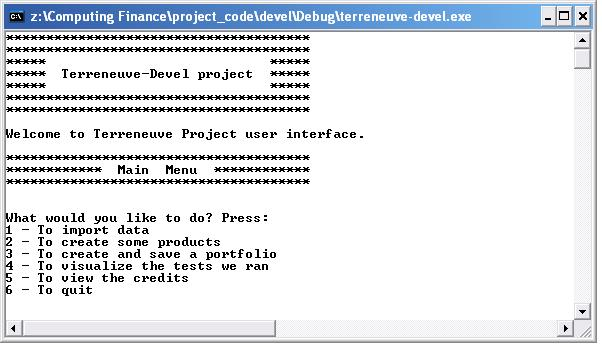
\includegraphics[width=11cm]{mainmenu.jpg}
        \caption{Main menu interface}
\end{center}
\end{figure}

From there he can 
\begin{enumerate}
	\item Import some data -- required for the options 2 and 3, the user can import our default data if he wants.
	\item Create some products -- all except the variance swap.
	\item Create/Retrieve a portfolio of all the products -- not available, but uses the option 2: all the existing menus to create a product in (2) return the object they created, so the adding of this functionnality to the user menu would be quick.
	\item Have a look at the C++ hard coded tests the coders ran to check their objects.
	\item Credits -- what is a GNU module without this !
	\item Quit -- which is too soon ... 
\end{enumerate}

\section{Import }

The import menu is straight forward -- here the user has chosen the default data. Else he has a menu to input the directory in which he has the data. An help menu on the file formats we used is available. Note that if the user wants flat rates, credit spreads and volatility, he should import the default data, as in all the menus the program asks him once more if he wants to use the data or enter flat curves.

\begin{figure}[htbp]
\begin{center}
        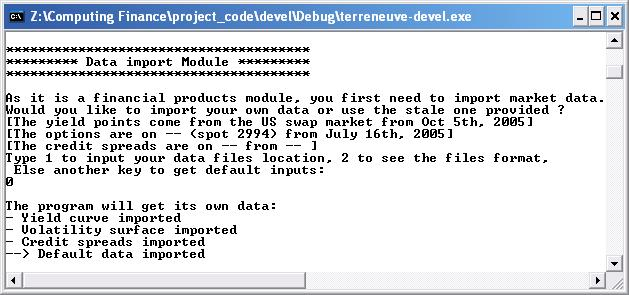
\includegraphics[width=12cm]{importDefault.jpg}
        \caption{Import data interface}
\end{center}
\end{figure}

\section{Products}

Once the import has been done, the user can create products and look at how they behave. If he wants to use flat curves, again he is being asked.

\begin{figure}[htbp]
\begin{center}
        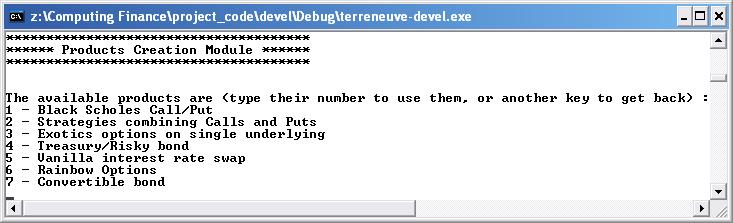
\includegraphics[width=12cm]{products.jpg}
        \caption{Products interface}
\end{center}
\end{figure}

The rest is very user friendly to create the products and view their sensitivities.


\section{Portfolio}

This has not been done in the menu, but as we said, it can be coded really quickly by using each product console input module and its functions:
\begin{enumerate}
	\item BlackScholes* inputBSOption(marketData data);
	\item OptionStrategy inputOptionStrategy(marketData data);
	\item Exotics* inputExoticOptionOnSingleAsset(marketData \&data);
	\item bond* inputBond(marketData \&data);
	\item VanillaSwap* inputVanillaSwap(marketData data);
	\item RainbowOption* inputRainbowOption(marketData data);
	\item convertiblebond* inputConvertibleBond(marketData \&data);
\end{enumerate}



\section{Credits}

Working together for 2 months leaves scars ... actually, it leaves anecdotes, so we tried to have the user share some of them.

Just select this option and you will see.




\section{Quit}

Come on, not yet, it is just the beginning of the report.

\chapter{Common objects}

\section{Date class}

Developer: Simon Leger

\subsection{Approach}

In order to work with financial data, where one of the most important factors is time, we 
needed a serious object to handle it.  This is why we came up with the idea of writing our own date class 
even if it was not really required in the project. This date class has been designed especially for financial use 
since one can find features common in finance such as business day and day count conventions.

In this approach the dates are stored as long integers where 1 is the first of January 1900.  Dates can also be easily created or accessed by giving the day, month and year. There is a whole set of powerful functions to get the last day of the month or to count the number of days 
between two dates according to a certain convention.

\subsection{Implementation}

There is a base class called Date and then a derived class called UsDate.  UsDate is able to use any function of the base 
class.  Additionally there is a boolean function which returns whether a specific day is a US business day or not. 
This could be adapted for any country by adding other sub classes.


\section{Interpolator}

Developer: Joseph Perez

\subsection{Approach}
We implemented a 1D and 2D quadratic interpolator.

The interpolator required for the implied volatility surface returns the degree two polynomial for each
maturity which best fits the computed implied volatilities.  However we can make two observations
\begin{enumerate}
	\item the shape of the surface of the S$\&$P now is a skewed surface more than a smile
	\item we want our interpolator to return a function that matches the known implied volatilities
\end{enumerate}
These requirements are not satisfied with the method described above.  Accordingly, we decided to implement another one. As the shape is rather smooth we do local interpolation: at a given point we evaluate the degree two polynomial which goes through the nearest known points. 


\subsection{Implementation}
We adapted the general implementation of polynomial interpolation from Numerical Recipes to focus only on polynomials of degree two.
In 1D, only one polynomial of degree two goes through three points. Our algorithm returns the evaluation of this polynomial on a fourth point without computing its coefficients.
In 2D, we use the same methodology. First we run three interpolations on one axis and then a last one on the other axis.

Outside our boundaries we force the interpolator to return the value of the nearest point.  This means that the interpolated curve or surface is flat outside the frontiers.

\section{Matrix}

Developer: Yann Renoux

\subsection{Approach}

Though we have decided to manage our data with valarrays to avoid dealing with pointers, the use of a matrix class was justified by two important applications in the yield curve and rainbow option sections of the project.

\subsubsection{The yield curve}

As part of the requirements for constructing the yield curve, we had to transform the swap rates into zero coupon rates in order to have an homogeneous set of points and be able to back out all the needed methods that a yield curve should have (most importantly spot rate to maturity, discount factors, forward rates). As shown in the yield curve section, changing from swap rates to zero coupon rates requires inverting a lower triangular matrix. Since coding the Gauss method for valarrays did not really make sense, a matrix class, based on Tony Veit's class was added to the project. Indeed, for such a basic tool, there is no need to re-invent the wheel. This class provides all the necessary methods and more to handle matrices generally.  Specifically, it made it easier to invert the swap rates matrix to get the zero coupons.

\subsubsection{Dealing with correlations - Cholesky decomposition}

On the section on rainbow options, we have to deal with correlated Brownian motions (see this section for more details). Though the formula is straightforward for a set of two underlyings, we aimed at making our classes as reusable as possible which motivated us to support more than two underlying assets.  The main issue was to sample $n$ independent normal distributions and recorrelate them all at the same time to produce correlated asset prices. One method to accomplish this is Cholesky decomposition of the correlation matrix. This method transforms a square matrix into a product of a lower triangular matrix multiplied by its transpose based on the eigenvalues decomposition without having to solve for them. Therefore, we added the Cholesky algorithm to the existing matrix class to be able to use it in the rainbow options class.


\subsection{Implementation}

There is nothing magic in this matrix class, it just has a double** as a private member to store the data, and then provides all the usual operators (redefined) for linear algebra, such as multiplication by a scalar or a matrix, transposition, inversion, etc. Additionally, the sum of columns, rows, diagonal matrix are available, as well as a "$<<$" operator to output the matrix. This was really useful in verifying the Cholesky decomposition results against what we expected.


\section{Cummulative bivariate normal distribution}

Developer: Yann Renoux

\subsection{Approach}

The rainbow options closed formulas need to use the Cummulative bivariate normal distribution function. The same way we ahve used the polynomial approximation, we have computed the polynomial approximation for $\mathcal{BN}(a,b,\r)$. We have used the approach discribed in Hull's \textit{Options, Futures and Other Derivatives - 5th Edition}, pages 245-246.

\subsection{Results and effects of the correlation}

The correlation mainly impacts the inflexion point steepness around $(a,b)=(0,0)$ as the polynomial approximation is a Taylor expansion. The more the correlation the steeper the inflexion point. The results are as follows:

\begin{figure}
\begin{center}    
        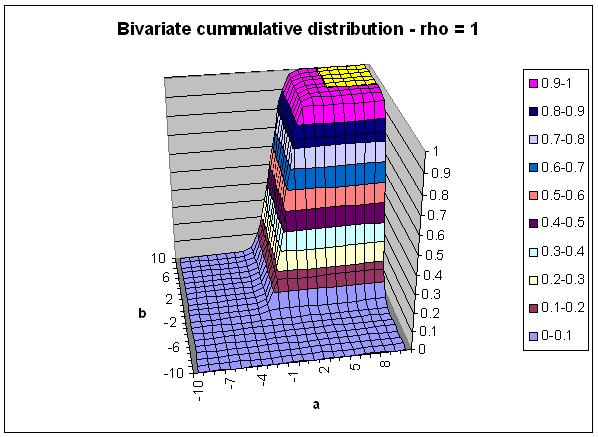
\includegraphics[width=10cm]{Bivn1.jpg}
        \caption{Cumulative bivariate normal distribution for $\r=1$}
\end{center}
\end{figure}

\begin{figure}
\begin{center}    
        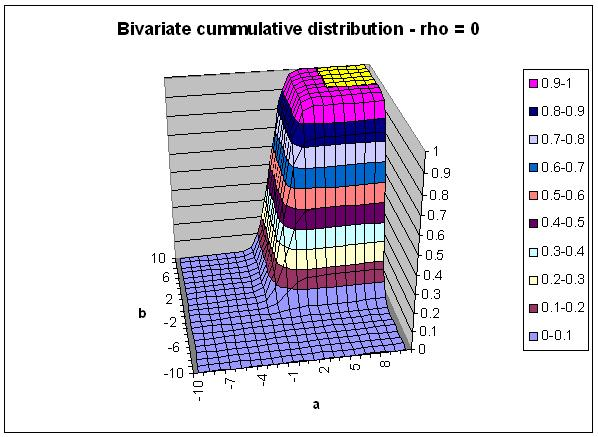
\includegraphics[width=10cm]{Bivn0.jpg}
        \caption{Cumulative bivariate normal distribution for $\r=0$}
\end{center}
\end{figure}

\begin{figure}
\begin{center}    
        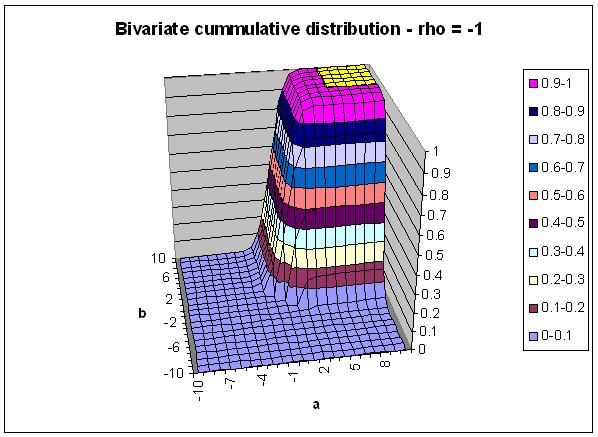
\includegraphics[width=10cm]{BivnNeg1.jpg}
        \caption{Cumulative bivariate normal distribution for $\r=-1$}
\end{center}
\end{figure}


\newpage

\section{FileReader}

Developer: Aloke Mukherjee

\subsection{Approach}

The FileReader class simplifies the task of working with structured data.  Some examples of structured data used in the project include swap and zero rates, option prices and credit spreads.  We wanted to be able to store this data in a simple comma-delimited text format so that it could be easily changed in a text editor.  The FileReader bridges the gap between this human-readable format and the data structures used in the project.  

\subsection{Implementation}

The FileReader relies on the CSVParser class developed by Mayukh Bose to read comma-delimited files.  Reusing this class allowed us to avoid some of the headaches involved with parsing text.  The CSVParser class has a simple but powerful interface that pipes in data from the file and pipes it out as an appropriate data type.  Some customization was required to allow the CSVParser to understand terreneuve-specific types like dates, credit spread types.  Once the data has been transformed from text into valid data types, FileReader can construct the internal data structures which are required to instantiate classes such as credit curves or a volatility surface.  

The other useful function of FileReader is discovering and caching the location of the common data directory.  The test routines use the cached value to locate their test data files.

\chapter{Part A: Black-Scholes and Monte Carlo pricer}
Developer: Simon Leger

\noindent Validator: Aloke Mukherjee


%DEVELOPER WRITES THIS PART --->

\section{Requirements}

%<description of the problem being solved, relevant equations, algorithms, etc>
In this section, we write a model to price European options using
the Black-Scholes formula and return the greeks associated to
these options. We also write a monte carlo pricer to be able to
check the prices for these options.

The formula for European options is depending on the type of the
options (i.e. Call or Put) is :
$$C(S,T)=S\mathcal{N}(d_1)-Ke^{-rT}\mathcal{N}(d_2)$$
$$P(S,T)=Ke^{-rT}\mathcal{N}(-d_2)-S\mathcal{N}(-d_1)$$
where :
$$d_1=\frac{ln(S/K)+(r+\sigma^2/2)T}{\sigma \sqrt{T}}$$
$$d_2=\frac{ln(S/K)+(r-\sigma^2/2)T}{\sigma \sqrt{T}}$$

and the greeks are :

\begin{center}
\begin{tabular}{|c|c|c|}
\hline
    {\bf } & {\bf Calls} & {\bf Puts} \\
\hline
{\bf delta} &     {$\mathcal{N}(d_1)$} &     {$\mathcal{N}(d_1)-1$} \\
\hline
{\bf gamma} & \multicolumn{ 2}{|c|}{{$\frac{\phi(d_1)}{S\sigma \sqrt(T)}$}} \\
\hline
{\bf vega} & \multicolumn{ 2}{|c|}{${S\phi(d_1)sqrt(T)}$} \\
\hline
{\bf theta} &     {$-\frac{S\phi(d_1)\sigma}{2sqrt(T)}-rKe^{-rT}\mathcal{N}(d_2) $} &     {$-\frac{S\phi(d_1)\sigma}{2sqrt(T)}+rKe^{-rT}\mathcal{N}(-d_2)  $} \\
\hline
 {\bf rho} &     {$KTe^{-rT}\mathcal{N}(d_2)$} &     {$-KTe^{-rT}\mathcal{N}(-d_2)$} \\
\hline
\end{tabular}
\end{center}

We then extend the previous model to provide the same results for
the following strategies :
    - Long Call Spread
    - Long Straddle
    - Long Butterfly Spread

\section{Design }

We have two folders for this part : one named BlackScholes which contains
the BlackScholes class which represents one european option and an OptionStrategy class
which is basically a portfolio of such options and provide important methods for them
as an easy way to create some options inside.


\section{Approach}
%<high-level description of the design>
To construct this, we see two important parts :
\begin{itemize}
    \item One pricer using formula
    \item A generic pricer using Monte Carlo approach
\end{itemize}

One class (named Black-Scholes) computes the prices, implied vol and
greek letters for a given type of option (type is either Call or
Put) and all this should be easily used through a nice
OptionStrategy class which is basically a portfolio of options. In
this class you have the ability to add options by giving their
parameters or use friendly methods that construct for you some
famous combinations, as has been specified in the requirements.

Then we build a multiple-class based monte Carlo pricer which is
driven by the MCEngine class. This pricer should be general enough
to price various derivatives products as it generates a path for
given dates, by taking into account the yield curve and the
volatility surface built in this project, hence the possibility to
price asian, look back options, etc.


\section{Choices}
%<any important design choices you made, e.g. data structures, class hierarchy, algorithm, etc. and a justification for the decision>
\par We did not choose to use polymorphism for the black-Scholes and
option strategy parts as both could be considered independent and
use separately.

\par For the Monte Carlo pricer we used polymorphism in order for the user
to be able to use different random number generators and still have
a robust interface Random class. The default number generator is
Sobol which is better than the default number generator of C++ and
provides enough numbers to be generated if required.

\par In addition, the user has a drift class that can be modified
easily to adopt other path generators. This one uses the extended
Black-Scholes model by taking into account the yield curve and the
volatility surface so they are not considered constant through the
path, which is useful for path dependent options.

\par Then there is a GaussianProcess class which takes the lognormal
process by adding the drift and the random numbers generated and
applying the corresponding volatility.

\par The Payoff class provides methods to take the path generated and
the strike and returns the payoff according to the option
specified.

\par There are four different sorts of number generators : the C++
default generator, the Park Miller generator, the Mersenne Twister
generator and also Sobol which is a quasi random generator. Here is
a comparison of precision for the different number generators : we
try to price a european call, the exact price being 4.94387 :
\bigskip

\begin{tabular}{|r|cc|cc|cc|cc|}
\hline
           & \multicolumn{ 2}{|c|}{300k} & \multicolumn{ 2}{|c|}{1M} & \multicolumn{ 2}{|c|}{10M} & \multicolumn{ 2}{|c|}{50M} \\
\hline
 Generator &      Price &       Time &      Price &       Time &      Price &       Time &      Price &       Time \\

     RandC &       4.96 &      2.156 &      4.935 &      7.172 &     4.9432 &      70.98 &     4.9461 &     355.62 \\

ParkMiller &      4.987 &      1.968 &      4.962 &      6.532 &     4.9448 &       67.7 &     4.9446 &     324.09 \\

MersenneTwister &      4.936 &      1.984 &      4.949 &      6.547 &     4.9461 &      65.08 &     4.9435 &     325.73 \\

     Sobol &    4.94354 &       1.95 &    4.94372 &       6.42 &    4.94385 &      64.26 &    4.94387 &     319.95 \\
\hline
\end{tabular}

\bigskip

As we can see, Sobol is way above the other generators for this kind
of test. Obviously the goal of a monte carlo number generator is to
try to fit at best the interval [0,1] and for this a quasi number
generator is much better than any pseudo generator. The only point
is that the numbers are less random from a general point of view,
since anyone can predict the next number, which is also possible for
any algorithm but usually less easy. For 300,000 paths, we have the
same precision with Sobol, than with Mersenne Twister for 50 million
paths ! And Mersenne Twister is known as the best pseudo random
number generators.  To meet the same precisions as the other pseudo
generators, the C++ random number generator requires 5 times more
paths and it is slower.

\section{Unit tests}

%<short descriptions of each subtest>
The unit test for this part was to build a market environment with a volatility surface and a yield curve and to compute the price of a european call and then to check the price with the monte carlo pricer, after we checked some results with both online pricers and a pricer built in Excel with the closed formula given by the Black-Scholes model.

\section{Performance}

%<how can the performance of this component be sped up by 100%?>
We first implemented this pricer using double* instead of valarray$<$double$>$ and the performance was much better (almost two times faster). This is due to a fixed cost when you read a valarray due to the cast type, but we chose to keep the version with valarray for a better integration with the rest of the code and to make it uniform and easier to read.

Another point could be to test other quasi random number generators
to see if they are more accurate than Sobol, and also to make an
interface for these random number generators to allow a multi
dimensional generation for rainbow options for exemple. The
implementation of Sobol algorithm is done with calibration up to 6
dimensions but we didn't use it since the interface has been done
for one dimension generation.

The last but not least point is that especially in banks, where most
of computers have two processors, it is possible to design the code
so that it can use two threads to take advantage of the available
CPUs.  An easier way that we tested was to create two executable
files and run them on a same machine (dual core Intel processor
2.8Ghz), but in this case one has to be careful about the
initialization of the random number generators otherwise the price
would be the same on the two threads. After this, one just has to
take the average of these prices. This would improve the performance
by 80\%, and maybe up to 250\% with four threads on a machine with
two processors with hyperthreading but we couldn't do this test
since our dual core machine didn't have hyperthreading.

%VALIDATOR WRITES THIS PART --->

\section{Validation}

The closed form formulas for European Calls and Puts as well as the
Greeks Delta and Vega were coded in Matlab (see BS.M in the data
directory).  These were then used to validate the C++ output.  The
Matlab version of Black-Scholes is quite simple to implement since
there already exists functions to calculate the cumulative normal
distribution.

\begin{figure}[htbp]
\begin{center}
        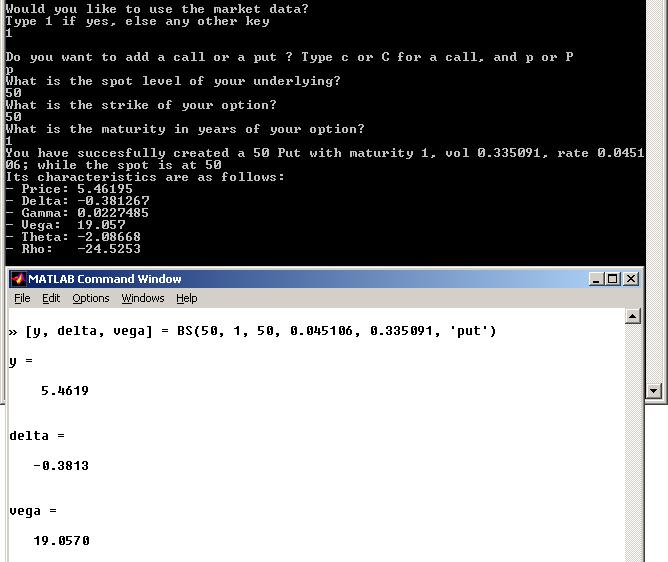
\includegraphics[width=12cm]{blackscholes-matlab.jpg}
        \caption{Verifying Put value with Terreneuve and Matlab}
\end{center}
\end{figure}

Another approach to validation was comparing with the results
obtained by the use of the binomial tree.  Since a binomial tree is
less accurate than the closed forms for European options the value
of this approach is debatable.  Nonetheless it was observed that the
binomial tree results were close to the closed form and Monte Carlo
solutions.

\begin{figure}[htbp]
\begin{center}
        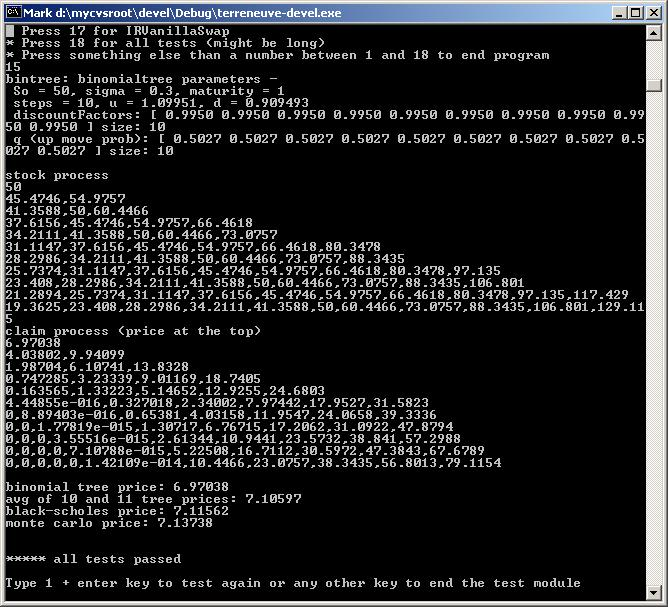
\includegraphics[width=12cm]{blackscholes-bintree.jpg}
        \caption{Comparing Black-Scholes and Monte Carlo Call value with Binomial Tree}
\end{center}
\end{figure}

\chapter{Part B: Yield Curve}
Developer: Yann Renoux

\noindent Validator: Joseph Perez


%DEVELOPER WRITES THIS PART --->

\section{Requirements}


\par All the formulas used in this project are based on risk-neutral valuation
and non-arbitrage, with a risk free rate. Hence whatever the product we consider,
we need to have a solid base class to handle the needs of classes that define products.
This object has to gather market data in the form of a market yield curve and provide the basic methods expected.
Such methods go from getting the spot zero coupon -- \emph{ZC} -- rate for a certain
maturity, the discount factor to present value future cash-flows or forward rates to evaluate
such future flows. But these methods can also include different interest composition, such as annual or continuous.

\subsection{Other methods we added for risk management purposes}

\par In addition to the basic methods required, we have added a shift and a rotation to model the 2 first
known factors of the Principal Component analysis on the term structure of a yield curve:

\begin{figure}
\begin{center}
        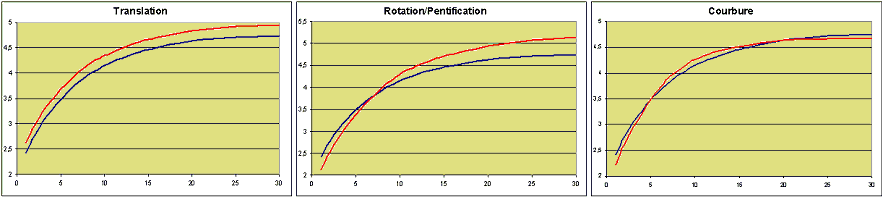
\includegraphics[width=12cm]{3mvts.png}
        \caption{3 first axis of the PCA (95\% of the variance): Shift, Rotation and Curvature}
\end{center}
\end{figure}


\par This will be very useful in term of risk management, as we know that all the rates bear a correlation and
the term structure is very unlikely to revert from one day to the other.

\par For instance, a yield curve is a set of data points with ascending maturities, related to some fixed-income product that provides a yield.
In practice, the short end of the curve comes from the ZCB's, and the rest is from the swap market. As those 2 evolve in a different space, the object needs to rotate the space of swaps into ZC rates.

\par We mentioned the methods we want the yield curve to be able to perform, but not what it will use as base data.
We have decided to store the term structure from the market curve, which is made
of zero coupon rates for short maturities -- 0.25, 0.5 and 1 year for the US market --
and swap rates -- from 2 to 10, 15, 20 and 30 years in the same market. As these rates do not come from the same
sort of product, they do not belong in the same space, hence a transformation needs to be done to have them in
comparable values: the class must be able to do the rotation transparently.

\subsection{From swap rates to ZC rates}
\par Consider a swap with notional $N$ such that:
\begin{itemize}
\item the floating leg delivers $m$ flows at dates $T_{j}$ for $j=1...m$
\item the fix leg with rate $C$ delivers $n$ flows at dates
$T_{ki}$ for $i=1...n$, $k$ being the ratio between the annual frequency of payment of the floating versus the fix leg, so that $kn=m$.
\end{itemize}

\par The so-called zero-coupons method provides a way to evaluate this vanilla swap, being equal to that of:
\begin{itemize}
\item a fixed coupon bond with same maturity and notional
\item minus the swap notional (a swap does not exchange principal).
\end{itemize}


\par Hence, defining $B(t,T_{ki}) $ the value at $t$ of a ZC paying 1 dollar at $T_{ki}$, we can write:
$$ SWAP_{t}=N \left(\sum_{i=1}^{n}C B(t, T_{ki})+B(t, T_{m}) \right)-N $$
where at any given date, the fix rate $C$ is the par swap rate, giving the NPV equal to zero.

\par Thus at $t$, each swap rate $s(t,.)$ verifies:
$$1=\sum_{i=1}^{m-1} \frac{s(t,m)}{\left(1+R(t,i)\right)^i} + \frac{1+s(t,m)}{\left(1+R(t,m)\right)^m}$$
Writing them up for all known maturities between 1 and $m$, we get matricially:

$$\left(
\begin{array}{ccccc}
1+s(t,1) & 0 & 0 &  & 0 \\
s(t, 2) & 1+s(t,2) & 0 & \ddots & \vdots \\
\vdots & \ddots & \ddots & & 0 \\
s(t,m-1) & & s(t,m-1)& 1+s(t,m-1)& 0 \\
s(t,m) & \cdots & \cdots & s(t,m) & 1+s(t,m) \\
\end{array}
\right) \left(
\begin{array}{c}
\frac{1}{\left(1+R(t,1)\right)^1} \\
\\
\vdots\\
\\
\frac{1}{\left(1+R(t,m)\right)^m} \\
\end{array}
\right)= \left(
\begin{array}{c}
1 \\
\\
\vdots\\
\\
1 \\
\end{array}
\right)
$$
that is to say:
$$ A(t) \left(
\begin{array}{c}
\frac{1}{\left(1+R(t,m)\right)^1} \\
\\
\vdots\\
\\
\frac{1}{\left(1+R(t,m)\right)^m} \\
\end{array}
\right)= \left(
\begin{array}{c}
1 \\
\\
\vdots\\
\\
1 \\
\end{array}
\right)
$$hence
$$\left(
\begin{array}{c}
\frac{1}{\left(1+R(t,1)\right)^1} \\
\\
\vdots\\
\\
\frac{1}{\left(1+R(t,m)\right)^m} \\
\end{array}
\right)= A(t)^{-1} \left(
\begin{array}{c}
1 \\
\\
\vdots\\
\\
1 \\
\end{array}
\right)
$$

\par Hence if we have all the intermediary points, we can just back out the ZC rates while solving an easy triangular system.
We will come back to the assumptions we made here later.


\section{Design }


\subsection{Approach}
%<high-level description of the design>
\par Prior to studying what a yield curve is, a simplier object should be defined, the yield point. Its 4 members are :
\begin{itemize}
    \item a type (Cash or Swap - but can be extended to other instruments),
    \item a rate,
    \item a maturity in years, and
    \item a Daycount convention (defaulted to Actual/360, the most common convention for USD Libor swap rates).
\end{itemize}
\par Note that the maturity is not a date, as commonly people talk about the 5 years swap rate or the 1 year ZC rate. The yield curve will be able to transform one into the other so that the user can use both.

\par A yield curve is then a valarray of yield points, but can be assigned a flat rate in anotehr constructor. At the construction, we need to make sure that the transformation is being made according to the method exposed earlier, so that the user can build a yield curve with several types of rates and be able to back out the tools without adding any line of code. In addition to that, the yield curve object also has a name field, so that the user can define a "USD Libor Curve" or a "EUR Libor Curve".

\subsection{Choices}
%<any important design choices you made, e.g. data structures, class hierarchy, algorithm, etc. and a justification for the decision>
\par As we said earlier, to get the ZC rates from the swap rates, we need to solve a triangular system. The 1 year swap rate is the 1 year zero coupon rate (write the formula...), but then it depends on what is the type of swap rate we are talking about. Say we have market quotes on semi annual swap rates, then we would need the 1.5 year swap rate to back out the 1.5 year ZC rate as we know the 1 year one. Here the choice was made to consider annual swap rates -- as in the Bloomberg quotes file provided, as well as a linear interpolation when needed. For instance, we have here solved the 1-10 years issue as all maturities there follow each other, but what for the rest ? Well the 12 years swap rate is taken as the weighted average of the nearest higher and lower rate known, here 15 and 10 years. We did not code splines interpolation method, as we thought that was not the main emergency in the class. As a result, we face a little bump on the reconstruction after the 10 year ZC rate due to this approximation:

\begin{figure}
\begin{center}
        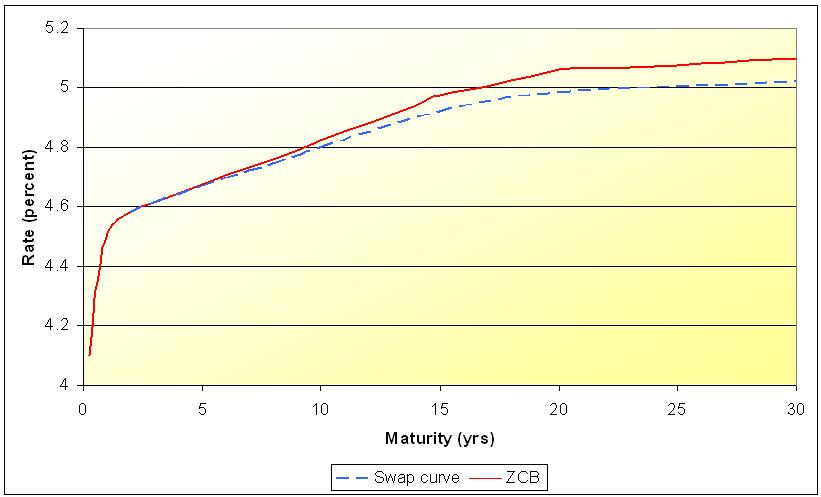
\includegraphics[width=12cm]{yc.jpg}
        \caption{ZC curve reconstruction from annual swap rates from 1-10 years, 15, 20 and 30 years.}
\end{center}
\end{figure}


\par We supposed that the user provides rates non ordered by maturity or type, then it does the sorting by itself. All the same if the user does not enter all rates, the swap to ZC private method does all what is needed to handle it.



\subsection{Methods}

\par On top of the necessay methods already mentionned (discount factor, forward rate, sorting, inverting swap to ZC, shift or rotate the curve, etc.), the yield curve has an output operator "$<<$" for easy checking, as well as a comparison one "==".

\subsection{Unit tests}

%<short descriptions of each subtest>
\par We used the file we provided from BBG (US Yield Curve "IYC", October, 5th, 2005). We computed zero coupons and output them as we saw earlier, computed some spot rates, discount factors, forward rates for different maturities in years or date, and changed the conventions. We have compared them to the calculus by hand in Excel, to make sure the results were coherent, as this class needs to be accurate for all the forthcoming ones.

\begin{figure}[htbp]
\begin{center}
        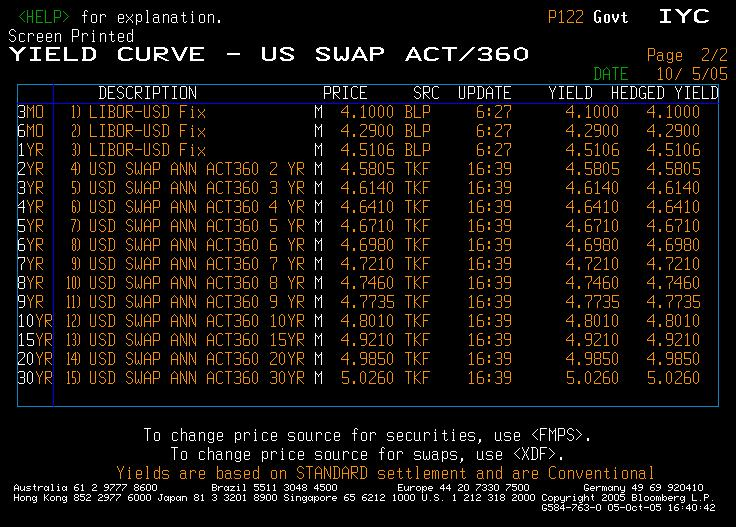
\includegraphics[width=10cm]{YC_RATES.jpg}
        \caption{Bloomberg YC Data for USA}
\end{center}
\end{figure}


\begin{figure}[htbp]
\begin{center}
        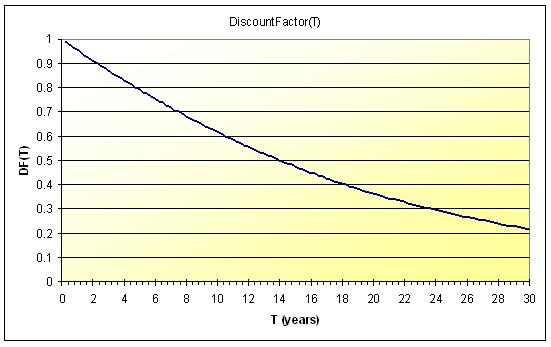
\includegraphics[width=12cm]{DF.jpg}
        \caption{Graph of the continuously compounded discount factors up to 30 years}
\end{center}
\end{figure}

\par We can note that the decreasing effect of the discount factor seems to be appropriate. See section 4. of the module to visualize the tests ran, as well as the validation part.

\begin{figure}[htbp]
\begin{center}
        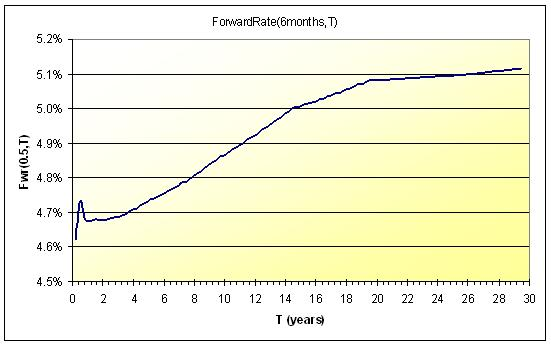
\includegraphics[width=12cm]{fwdRates.jpg}
        \caption{Graph of the forward rates starting in 6 months}
\end{center}
\end{figure}


\par On the forward rate graph, there is a break at (6m,6m) which corresponds to the change from ZC to swap rates, indeed the interpolation method has a huge impact on the forward rates. See \textit{http://www.riskworx.com/insights/interpolation/interpolation.htm} for more explanation. We conclude that for our purpose, the forward curve is satisfactory, and as mentionned, could be improved by improving the interpolation method.

\par To finish, we tested the several methods, spot, discount factor, forward rate and compared to the calculus we should have, just by using the yield curve and calculating the expected prices. They were all in line -- see the mainyieldcurve program in the test directory for more details. Results in in data/rates.xls

\subsection{Performance}

\par We have mentionned various assumptions, and their addition would increase the computation time. For instance, the flexibility of swaps frequency, or the splines interpolation.

\par But as is, aside of the valarray that might not be "the" efficient structure for a too small amount of data, some methods or storage could be improved. As an example, all the getSwapRates - maybe we could store them separately at the construction and avoid needing to find them, etc.
Also, the getSequentSwapRates, used to the first part of the curve 1Y-10Y, is used only to be able to know whether or not to interpolate. It might be redundant if the list of swaps we get for the matrix invertion was better seen.


%VALIDATOR WRITES THIS PART --->

\section{Validation}


\subsection{Approach}
A way to validate the construction of a yield curve was to compute prices of zero coupon bond of short maturity and the swap rates with a yieldCurve object and compare them to the input we gave to construct it. They matched.
The other validation method was to use the yield curve in every other section. As with the other objects (bond, montecarlo...) we got good results it means that the yield curve was well defined.
%\subsection{Pitfalls}

%<i.e. what bugs were found>

\chapter{Part C: Asset}
Developer: Yann Renoux

\noindent Validator: Joseph Perez


%DEVELOPER WRITES THIS PART --->

\section{Requirements}

\par This is an underlying asset class. It has a currency, a spot price level and a dividend
 schedule or a fixed dividend rate. It also possesses a yield curve, supposingly in his currency of denomination, which purpose is to discount future flows. We have made the choice not to use it as a member for the other classes, but it bears all the necessary information. It could be used as to provide a dividend growing rate for Black Scholes object for example.

Hence the choice has been made not to use an asset with a volatility surface that would simulate itself forward prices, as indeed it would be a single simulated price, and in expectation, the volatility does not enter into account.

The only purpose of this object is to be able to be added in the portfolio to hedge options on the book.

\section{Design }

\par Obviously a stock is a delta one security, the interesting thing is the benefit of carry with the dividends versus its cost of carry against the money we would get while depositing the money at the current market rate.

The other thing is that usually, with no inside information on the company, one cannot know for sure the future dividends that will be paid. Thus we decided to add the fixed dividend rate, which in practise would be an econometrically estimated parameter, but a very commonly used input in pricing, such as in Black-Scholes for instance.

The well-known formula for pricing a stock with dividends is:
\[
P_t=\sum_{i=1}^\infty Dividend_{t+i}\times DiscountFactor(t,t+i)
\]

Hence the forward price:
\[
F(t,T)=P_T=\sum_{i=1}^\infty Dividend_{T+i}\times DiscountFactor(t,T+i)
\]
In practise it would be the current price minus the known future dividends up to the date $T$. This entails and reflects the drop in price that a stock sustains when a dividend is paid: it theoretically decreases its current price by the exact amount that has been paid. On the contrary, with a fixed dividend rate $q$, the forward price is $F(t,T)=P_t e^{-q(T-t)}$. The following graph reflects this noticed fact.
\begin{figure}
\begin{center}
        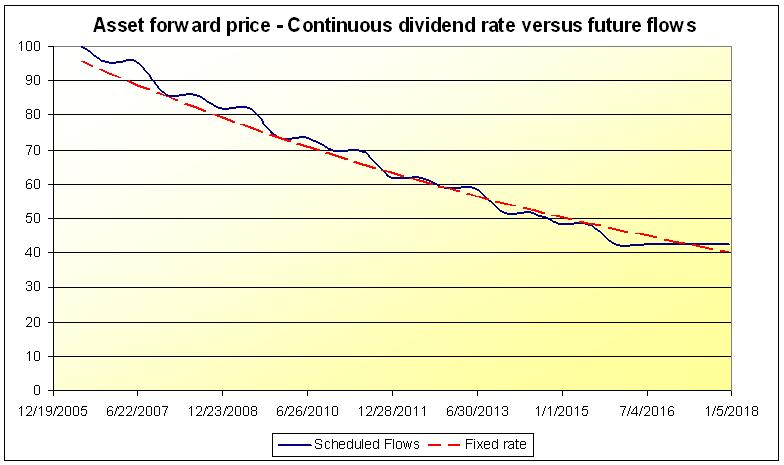
\includegraphics[width=12cm]{assetFWD.jpg}
        \caption{Asset forward price - comparison of a fixed continuous rate versus a dividend schedule}
\end{center}
\end{figure}

The continuous rate has been taken equal to $7.5\%$, while for the purpose of demonstration, the dividend schedule in the other case is up to 10 years, with $5\%$ the even years, and $10\%$ the odd years. The first noticeable fact is the sudden drop when the dividend is paid. This is not on an accrual basis as the bonds! On the other hand, the graph goes beyond the 10 years, and we remark that by then the forward price of the dividend scheduled asset remains constant, which is in agreement with the formula. Last note that the apparently increasing forward price is not the reality, it is just due to smoothing in Excel graph -- look at the output file produced by the test menu to check it.


\section{Approach}

\par The dividend schedule is a valarray of flowSchedule, a class with a date, an amount in percent, and a business day convention for the payment date. Indeed, if the payment date does not fall on a working day, the accrued interest calculation can differ depending on the convention.

An asset then has the mentionned members, should the user specify in the constructor the type of dividend, fix rate or scheduled. All the methods check this before pricing.


\section{Methods}

\par The forward price is using the formulas mentionned above, and the class has a getDelta function so that the portfolio class can know that holding an asset is delta one.

\par The getPrice method has been made virtual so that if later we want to inherit from this, we can do it.

\section{Unit tests}

\par We have tested several dividend rates, and schedules, checking that the forward drops on the payment date by the expected amount. The output file for the 10 year dividends illustrates well what we did.

\section{Performance}

\par This class being rather simple, nothing huge can be done to make it quicker. And if so, this was not at all the most important object to improve. See the mainasset in the test directory for more details.


\section{Validation}
No particular validation test were needed for this simple class, we just had to check that code had no bug and formula for forward price was correct.


\chapter{Part E: Implied volatility surface}
Developer: Joseph Perez

\noindent Validator: Simon Leger

%DEVELOPER WRITES THIS PART --->

\section{Requirements}

Giving a matrix of call and put prices for a range of maturities and strikes and a yield curve allows us to invert the Black-Scholes formula for each price to get the implied volatility.
In plotting the matrix of implied volatilites we create an implied volatility surface.

According to Black-Scholes option pricing model, the volatility for calls and puts for the same maturity should have the same volatility of the stock price and the implied volatility surface should be a term structure.
However market prices indicate that volatilities depend on strikes level.
The implied volatility surface of market prices looks like a smile.

\section{Design }

We build an implied volatility surface for an underlying from its price, a yield curve and a table of standard european call/put prices for different maturities and different strikes.

Black-Scholes' model makes it possible to price a call or a put with closed form solution if we consider constant volatility  and constant interest rate. But the classical option pricing formulas can be inverted and we can compute what is commonly call the implied volatility if we know the price.

According to Black-Scholes option pricing model, the volatility for calls and puts for the same maturity should have the same volatility of the stock price and the implied volatility surface should be a term structure.
However market prices indicate that volatilities depend on strikes level.
The implied volatility surface shape can be different depending on the underlying. Smile, smirk or sneer are kinds of name we give to caracterize those shapes. For equity index options markets, it is more of a skewed curve. This has motivated the name  "volatility skew".




European options on stock are often liquid and option prices are given by the market. We use for the price the midpoint of Bid/Ask.



\section{Approach}
%<high-level description of the design>

\section{Choices}
Once our price inverted we have a range of implied volatilites for different levels of strike and different maturities. Then we can get the implied volatity (or variance) for a given strike and a given maturity using a quadratic interpolation.
As the implied volatility surface is rather smooth a local 2D quadratic interpolation gives us good approximation.


\section{Methods}
For each maturity and each strike for which we have the price of a call or a put, we create a BlackScholes object. The constructor of BlackScholes class inverts Black-Scholes formula using the recursive Newton-Raphson algorithm in order to get the implied volatility.

Once the implied volatility surface is set we can compute the implied volatility (or variance) for any maturity and any strike.
To do this we use the 2D-quadratic interpolator.
As the surface is rather smooth and looks like a parabol, a quadratic interpolation gives us good approximation.

The class includs a method to compute a forward volatility. Assuming we built our implied volatility surface at time $t$ and we want to know what would look like the volatility at time $T_2$ seen at $T_1$ for a strike $K$. We use the following formula
\[
\sigma_{T_1,T_2}^2(K)=\frac{\sigma_{T_2}^2(K)(T_2-t)-\sigma_{T_1}^2(K)(T_1-t)}{T_2-T_1}
\]
%<brief descriptions of methods - can take from doxygen documentation>

\section{Unit tests}
We build the implied volatility surface for the S$\&$P500 from call and put prices of July 2004. The shape we get is as expected, it is a "skewed surface".
\begin{figure}
\begin{center}
        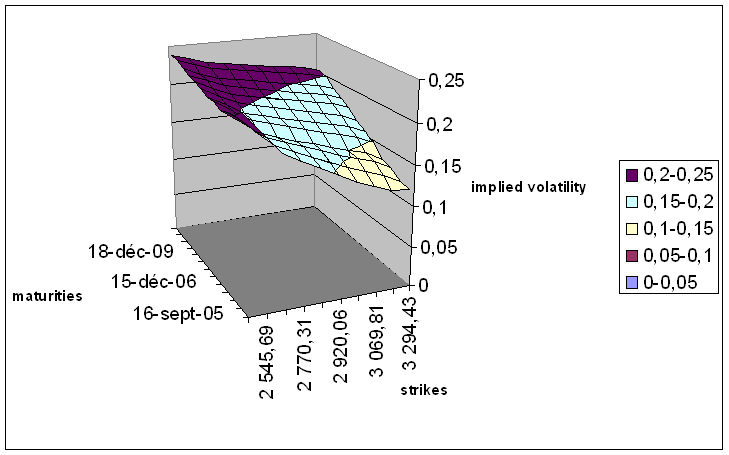
\includegraphics[width=12cm]{volsurfjoseph.jpg}
        \caption{Volatility surface of S$\&$P500}
\end{center}
\end{figure}

\section{Performance}

The Vega of call/put is always positive option prices are increasing function of the volatility that's why Newton-Raphson algorithm is accurate in this case. By default inversion of Blacks Scholes formula return the computed volatility after 100 iterations. In practice the volatility converges quickly, only 10 iterations are necessary. So we could either set the number of iterations to be 20 or to compare after each iteration the difference $|\s_{n+1}-\s_n|$ and exit the loop as it is inferior to a level $\epsilon$.

%VALIDATOR WRITES THIS PART --->

\section{Validation}


\subsection{Approach}

%<i.e. what alternate method was used to validate the results - if this required a lot of code then similar outline as above should apply>

To test this class, whose accuracy is very important for the rest of the project, we ran two tests. 
First we instanciated an object of the volsurface using the flat volatility constructor and we 
checked that every point was giving the same and correct volatility and we also checked the 
values of forward volatilities in an Excel spreadsheet by replicating the formula. 
\par Then we created a bench of strikes and dates in an Excel spreadsheet and by choosing a volatility 
for these points, just arbitrary. We compute the black scholes price for each of these options 
and we load these prices, dates and strikes into our c++ project and construct the yieldcurve with them. 
After this, we decide to get some volatility from this object for some strikes and matuirties and we check 
if they give exactly the same result than for the inputs and nice enough results for other points.
Then we simply plot the volatility surface in a two dimensional chart to check its shape.
\par Here is the table for these volatilities given the strikes and maturities transformed in years :

\noindent
\begin{tabular}{rrrrrrrrrrr}

  maturity &    2395.95 &    2545.69 &    2695.44 &    2770.31 &    2845.19 &    2920.06 &    2994.93 &    3069.81 &    3144.68 &    3294.43 \\

 0.1697467 &        0.2 &       0.19 &       0.18 &       0.17 &       0.16 &       0.15 &       0.14 &       0.13 &       0.12 &       0.11 \\

 0.6680356 &       0.22 &       0.21 &        0.2 &       0.19 &       0.18 &       0.17 &       0.16 &       0.15 &       0.14 &       0.13 \\

 1.4154689 &       0.24 &       0.23 &       0.22 &       0.21 &        0.2 &       0.19 &       0.18 &       0.17 &       0.16 &       0.15 \\

 2.4312115 &       0.26 &       0.25 &       0.24 &       0.23 &       0.22 &       0.21 &        0.2 &       0.19 &       0.18 &       0.17 \\

 4.4243669 &       0.28 &       0.27 &       0.26 &       0.25 &       0.24 &       0.23 &       0.22 &       0.21 &        0.2 &       0.19 \\

 7.4332649 &        0.3 &       0.29 &       0.28 &       0.27 &       0.26 &       0.25 &       0.24 &       0.23 &       0.22 &       0.21 \\

\end{tabular}  
As one can see we constructed a linear volsurface, increasing with maturity and decreasing with strike, and here is the plot of this surface :

\begin{figure}
\begin{center}
        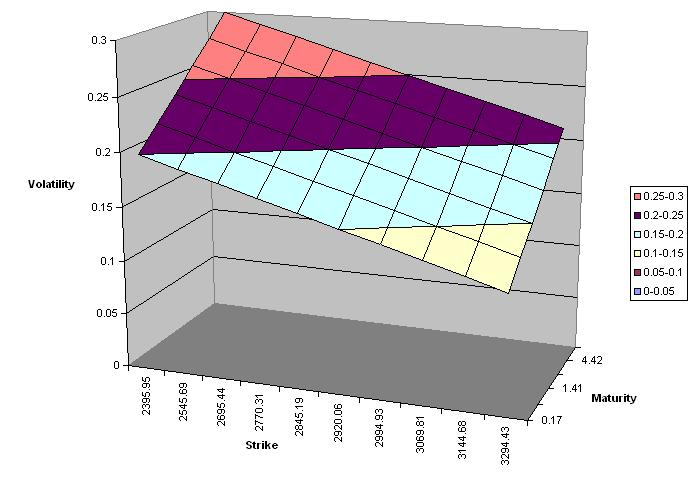
\includegraphics[width=12cm]{volsurf1.jpg}
        \caption{Linear Volatility surface}
\end{center}
\end{figure}


\chapter{Part F: Credit Curve}
Developer: Aloke Mukherjee

\noindent Validator: Yann Renoux


%DEVELOPER WRITES THIS PART --->

\section{Requirements}

%<description of the problem being solved, relevant equations, algorithms, etc>
A credit curve is similar to a yield curve in that it can be used to
calculate discount factors and thus present or future values of a
risky security.  The key difference is that there is a spread at
each maturity between the credit curve and the yield curve
corresponding to the additional return required for taking on the
added risk.

Credit curves are associated with the issuer's creditworthiness.
There is always a probability that the issuer will default and thus
be unable to meet their debt obligations.  A survival probability
quantifies the probability at any given time that the issuer will
"survive" to meet these obligations.  Survival probability declines
with time and declines faster for less credit-worthy issuers.

We calculate implied probabilities from credit default swap spreads.
In a credit swap the buyer of protection pays the spread
periodically and the seller pays in the event of a default.  These
two legs must have equal present values.  The assumption underlying
this model is that the spread on a risky asset vs. a non-risky asset
is entirely compensation for the possibility of default.  The
CreditCurve class models the modified yield curve as well as the
issuer's survival probability, hazard rate and recovery rate.

\section{Design }

All of the discounting functionality can be reused from the
YieldCurve object.  The CreditCurve object must also maintain a
collection of spread points.

The more interesting part of the implementation was bootstrapping
the default probabilities.  We decided to implement the calculation
recursively.  We define the following terms:

$q_{n}$ - default intensity.  This is the probability of default in
period n conditional on no earlier default.

$Q_{n}$ - default probability.  This is the probability of default in
period n as seen from time 0.

$S_{n}$ - survival probability.  This is the chance of survival to
time n.

$C_{n}$ - cumulative default probability.  This is the chance of
default before time n.  It is the complement of $S_{n}$.  This value
is called $Q_{n}$ in Professor Laud's notes.

$F_{n}$ - fees associated with one leg of a credit default swap.
Both legs are assumed equal to this value so the quantity can be
computed either from the perspective of the buyer or seller of
protection.

$B(0,t_{n})$ - discount factor.  The value of one dollar received at
time $t_{n}$.

$s_{n}$ - spread.  The credit spread over the riskfree rate at
time n.

$R$ - recovery rate.  The proportion of face value recovered in
the event of default.  It is usually assumed to be 40\%.

The following relationships hold for these quantities:

$$q_{0} = 0, q_{1} = Q_{1}$$

$$Q_{2}=(1-q_{1})(q_{2}) \Rightarrow Q_{n} = (\prod_{i=1}^{n-1}(1-q_{i}))q_{n}$$

$$S_{n} = 1 - \sum_{i=1}^{n}Q_{i} = \prod_{i=1}^{n}(1 - q_{i})$$

$$C_{n} = 1 - S_{n} = \sum_{i=1}^{n}Q_{n}$$

Generalizing from the risk-neutral argument of equality between swap
legs at each default time we can write down the following recursive
formula for $q_{n}$ in terms of fees $F_{n}$, survival probabilities $S_{n}$, spreads $s_{n}$,
recovery rate $R$ and appropriate discount factors:

$$q_{n}=\frac{F_{n-1}(\frac{s_{n}}{s_{n-1}} - 1) + B(0,t_{n}) s_{n} S_{n-1}}{B(0,t_{n}) S_{n-1} (1 - R + s_{n})}, q_{0} = 0 (probability\ of\ default\ at\ time\ 0\ is\ 0\%)$$

$$S_{n}=S_{n-1} (1 - q_{n}), S_{0} = 1 (probability\ of\ survival\ at\ time\ 0\ is\ 100\%)$$

$$F_{n}=F_{n-1} \times \frac{s_{n}}{s_{n-1}} + B(0,t_{n}) s_{n} S_{n-1} (1 - q{n})$$

$$F_{0} = 0 (no\ fees\ at\ time\ 0)$$

By implementing recursive methods for default probability, survival
probability and fees we can calculate default intensities at
discrete time intervals.  Notice that all the above is considered in
the discrete time setting for simplicity of implementation and
because of the discrete nature of the spread data.

\section{Choices}
%<any important design choices you made, e.g. data structures, class hierarchy, algorithm, etc. and a justification for the decision>

There are three choices with respect to reuse of the YieldCurve
class.  CreditCurve can inherit from YieldCurve, YieldCurve and
CreditCurve could both inherit from some common class or CreditCurve
could contain a YieldCurve.

The first two have the benefit of allowing polymorphism - e.g. a
function designed to take a YieldCurve object and use it for
discounting can also take a CreditCurve object.  This would not be
possible in the third case unless there were some method of
CreditCurve which returned a YieldCurve.  This is cumbersome.  Of
the two polymorphic approaches the first has the benefit of
simplicity and intuitiveness: namely there is no object more basic
than a YieldCurve in finance and secondly the CreditCurve is a type
of YieldCurve rather than a type of some other more basic object.
Our implementation takes the first approach.

In calculating default probabilities we decided to throw out the .5
year spread since keeping it requires having a special case. Instead
we standardize the calculation on 1 year intervals - i.e. we assume
that defaults happen at the 1/2 year mark.  Another justification
for this is that looking at the sample data we received for AIG from
Bloomberg, it appears that the .5 year spread is interpolated (equal
to 1 year spread).


\begin{figure}
\begin{center}
        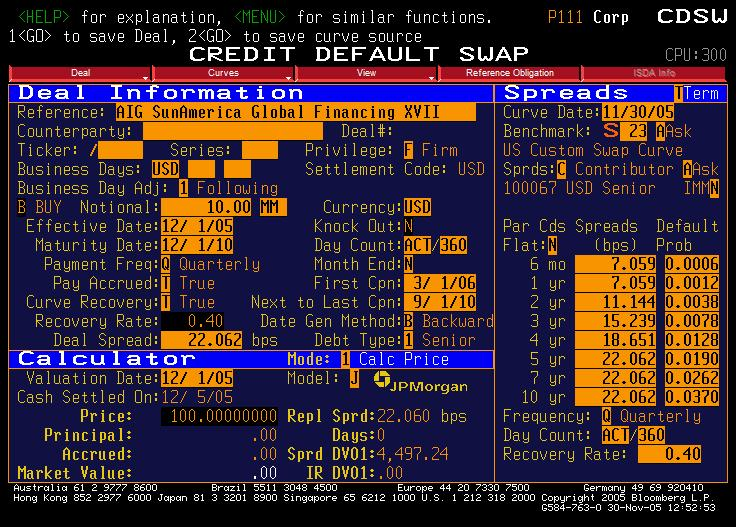
\includegraphics[width=10cm]{CDSW_AIG.jpg}
        \caption{Bloomberg CDS data for AIG}
\end{center}
\end{figure}

We also decided to internally interpolate spreads at 1 year
granularity rather than working with discontinuities in the spread
data.  Hull suggests one approach for calculating default
probabilities on an interval where there is no spread data: assume a
constant unconditional default probability in each period.  Since
the calculations implemented here work with conditional default
probabilities it is easier to assume a spread and leave the
calculation as it is.  From the rough relationship $$h =\frac{s}{(1-R)}$$ 
we know that spreads are proportional to
conditional default probabilities.  So interpolating spreads is like
assuming a constant default probability in the interval.  The
approach of using a constant default intensity is suggested in
section 21.3 of OFOD (6th edition). For another supporting argument
for this approach see
http://www.fincad.com/newsletter.asp?i=1140\&a=1800 which suggests
interpolating CDS spreads as an improvement vs. constant "default
density" (a.k.a. unconditional default probabilities).

The risky discount factor was calculated by multiplying the
underlying riskfree discount factor by the discrete time survival
probability up to that time rather than using a continuous
hazard-rate function.  In the class notes we have $RF = DF \times
(1 - Q(T))$.  $Q(T)$ is cumulative default probability (in
Professor Laud's notes, here we denote it $C_{n}$) so it is the
complement of $S(T)$, the cumulative survival probability.

In discrete time we have the identity: $\frac{(S_{n} -
S_{n+1})}{S_{n}} = q_{n}$.  $q_{n}$ is a discrete time version of
hazard rate.  In the limit this leads to the expression $S(t) =
exp(-\int_0^th(t)dt)$.

The risky discount factor is a "discounted" discount factor - the
discounting applied is the survival probability. In continuous time
we can use the expression above but since we have calculated
everything to this point in discrete time and we have an explicit
expression for the survival probability we use this as the discount
factor rather than the continuous time expression above.

\section{Unit tests}
%<short descriptions of each subtest>

The recursive algorithm was first implemented in Matlab.  The
M-files can be found in the data directory: $$defprob.m, survprob.m,
fees.m$$ Using Matlab some of the results in section 21 of OFOD
were successfully reproduced.  When implemented in C++ the results
were verified against the Matlab output as well as the example in
OFOD.  Another source of verification was the reuse of the credit
curve class in implementing the risky bond.

Additionally the given data for AIG was encoded in a file and used
to instantiate a CreditCurve.  The data was gathered using
CreditCurve's appropriate methods and plotted here and on the
following pages. The cumulative default probability curve comes
quite close to the Bloomberg curve.

\begin{figure}
\begin{center}
        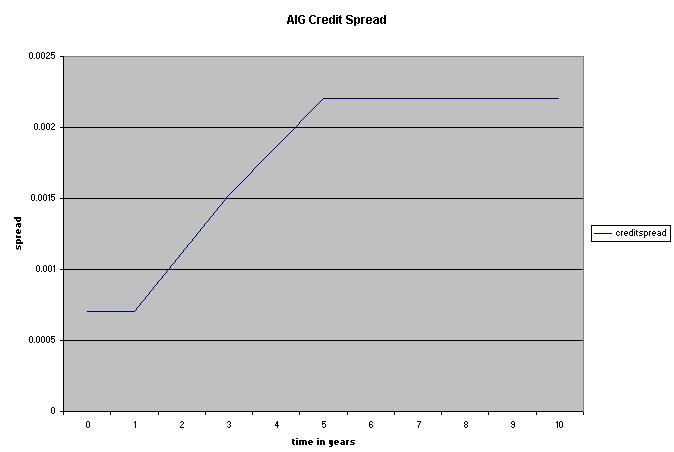
\includegraphics[width=10cm]{creditcurve-spread.jpg}
        \caption{Credit spreads}
\end{center}
\end{figure}


\begin{figure}
\begin{center}
        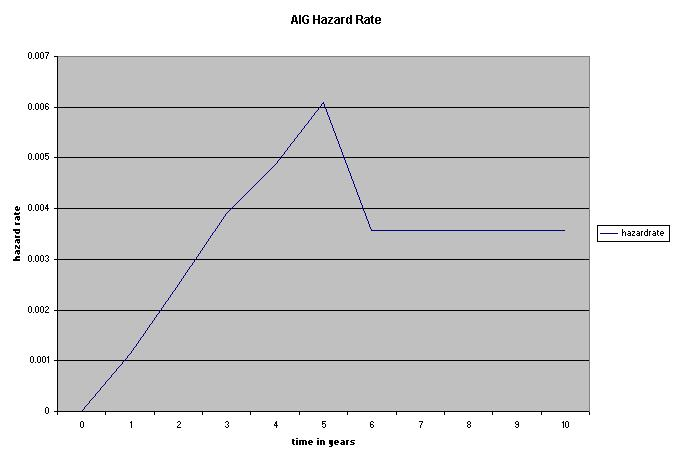
\includegraphics[width=10cm]{creditcurve-hazardrate.jpg}
        \caption{$q_{n}$ - hazard rate or default intensity}
\end{center}
\end{figure}


\begin{figure}
\begin{center}
        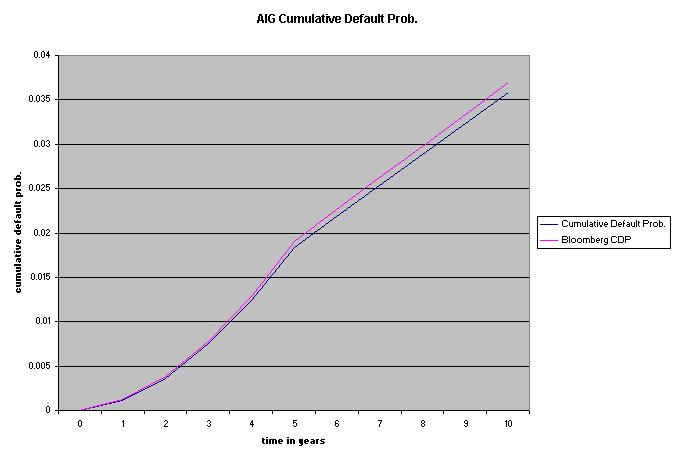
\includegraphics[width=10cm]{creditcurve-cumdefaultprob.jpg}
        \caption{Comparison between calculated and values from Bloomberg}
\end{center}
\end{figure}

\begin{figure}
\begin{center}
        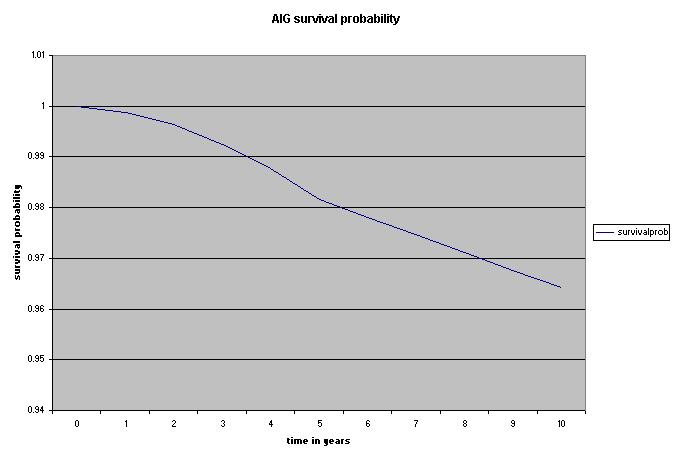
\includegraphics[width=10cm]{creditcurve-survivalprob.jpg}
        \caption{Survival probability}
\end{center}
\end{figure}

\begin{figure}
\begin{center}
        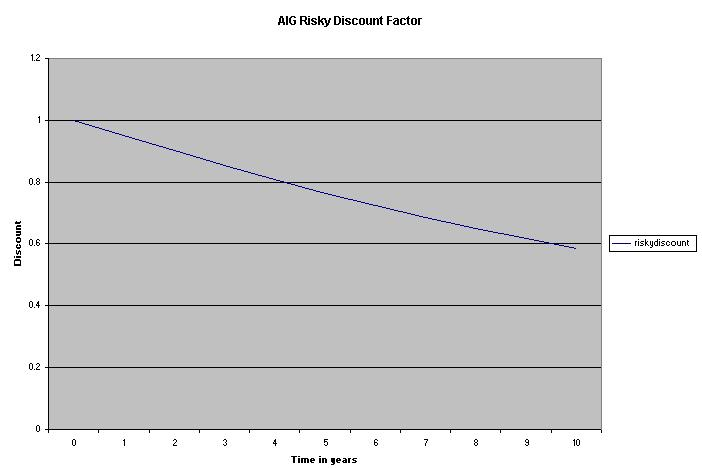
\includegraphics[width=10cm]{creditcurve-riskydiscount.jpg}
        \caption{The risky discount factor}
\end{center}
\end{figure}

\section{Performance}

%<how can the performance of this component be sped up by 100%?>
Recursion can be time-consuming resulting in many nested calls.  One
approach to improving performance is to cache intermediate results.
Caching was implemented and makes the performance O(n) for the first
call (assuming you are calculating default probabilities from
earlier to later periods).  Once all values are cached, results are
immediate.  Overhead for the first call could be further reduced if
the values were cached at construction.

The best candidate for performance improvement in the CreditCurve
class is probably the method used to construct the curve.  The
spreads are all converted to relative spreads and then used to
construct a new yield curve. Then the spotrates of the underlying
curve and the "spread curve" are summed to instantiate a combined
curve.  This procedure is a bit overly time and memory consuming and
could be optimized.

%VALIDATOR WRITES THIS PART --->

\section{Validation}


\subsection{Approach}

We applied the algorithm present in Pr. Laud lecture notes. Define
\begin{itemize}
    \item A spread $sprd_T$ is paid annually constantly to protect for the default during $T$ years.
    \item $q_i =q(i-1,i)$ is the conditional probability of default in period i. $q_0=1$
    \item $Q(i)$ is the cumulative probability such as $Q(0)=0$ and $Q(i+1)=Q(i)+q_{i+1}[1-Q(i)]$
\end{itemize}

To compute we note that the Present Value of the fees on the whole
life should equal the loss occurred in case of default, all been on
the point of view of the seller. If we call $B(0,j)$ the risk free
discount factor up to year $j$ and $R$ the recovery rate:

\begin{eqnarray*}
    \mathbb{E}(PVFees,T)&=&sprd_T\times\sum_{i=1}^T\left(B(0,i)\prod_{j=1}^i(1-q_j)\right)\\
    \mathbb{E}(Loss,T)&=&(1-R)\times\sum_{i=1}^T\left(q_iB(0,i)\prod_{j=1}^{i-1}(1-q_{j})\right)\\
\end{eqnarray*}

The first conditional probability is easy to compute, and we used Excel's "Goal Seek" to find recursively the conditional probabilities that would equal the fees and the loss. We repeated this for 5 years -- credit spreads were provided by the developper and we used the default yield curve, and were led to the $Q(i)$ which are used to get the risky discount factor. The results are as follows:

\begin{center}
\begin{tabular}{|l|l|l|l|l|l|l|}
\cline{3-7}
\multicolumn{1}{l}{} & \multicolumn{1}{c|}{} & \multicolumn{3}{c|}{Values of Q(i) computed with several tools} & \multicolumn{2}{c|}{Relative Differences between Q(i)'s} \\
\hline
Yr & \multicolumn{1}{c|}{creditspread} & \multicolumn{1}{c|}{Terreneuve} & \multicolumn{1}{c|}{Excel} & \multicolumn{1}{c|}{BBG (Interpolation)} & \multicolumn{1}{c|}{Excel/Bloomberg} & \multicolumn{1}{c|}{ Excel/TN} \\
\hline
$1$ & \multicolumn{1}{c|}{$0.00071$} & \multicolumn{1}{c|}{$0.00115$} & \multicolumn{1}{c|}{$0.00118$} & \multicolumn{1}{c|}{$0.0012$} & \multicolumn{1}{c|}{$2.1\%$} & \multicolumn{1}{c|}{$2.4\%$} \\
\hline
$2$ & \multicolumn{1}{c|}{$0.00111$} & \multicolumn{1}{c|}{$0.00365$} & \multicolumn{1}{c|}{$0.00374$} & \multicolumn{1}{c|}{$0.0038$} & \multicolumn{1}{c|}{$1.6\%$} & \multicolumn{1}{c|}{$2.4\%$} \\
\hline
$3$ & \multicolumn{1}{c|}{$0.00152$} & \multicolumn{1}{c|}{$0.00754$} & \multicolumn{1}{c|}{$0.00772$} & \multicolumn{1}{c|}{$0.0078$} & \multicolumn{1}{c|}{$1.0\%$} & \multicolumn{1}{c|}{$2.3\%$} \\
\hline
$4$ & \multicolumn{1}{c|}{$0.00187$} & \multicolumn{1}{c|}{$0.01237$} & \multicolumn{1}{c|}{$0.01266$} & \multicolumn{1}{c|}{$0.0128$} & \multicolumn{1}{c|}{$1.1\%$} & \multicolumn{1}{c|}{$2.3\%$} \\
\hline
$5$ & \multicolumn{1}{c|}{$0.00221$} & \multicolumn{1}{c|}{$0.01839$} & \multicolumn{1}{c|}{$0.01881$} & \multicolumn{1}{c|}{$0.0190$} & \multicolumn{1}{c|}{$1.0\%$} & \multicolumn{1}{c|}{$2.2\%$} \\
\hline
\end{tabular}
\end{center}

The differences are not very important, as in relative value $2\%$, but still significative. Neither TN nor Excel matches Bloomberg results, which explains by the fact that we did not have the yield curve of the same day of quotation of the CDS. We still have to mention that Excel seems closer to Bloomberg, but that TN results are far from being off, so the class can be validated as it is and consider giving a fair result for all the objects that use it. Once this works, the formulas exposed before follow form one another.

\begin{figure}
\begin{center}
        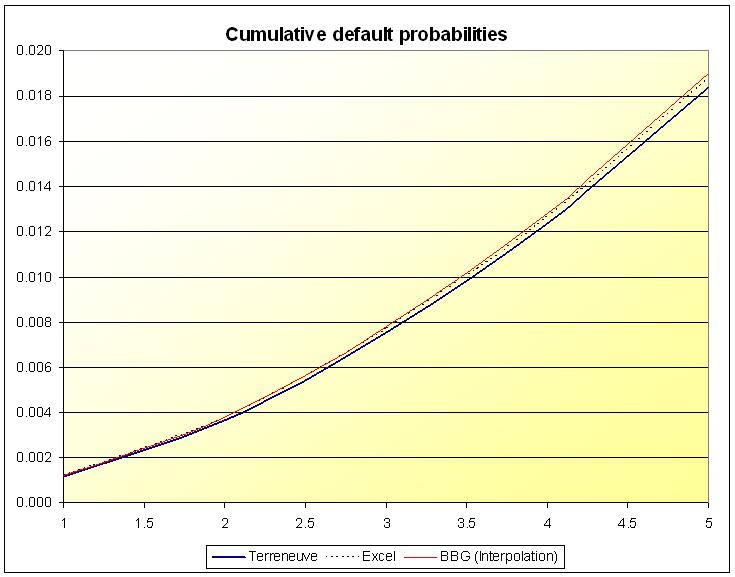
\includegraphics[width=14cm,height=10cm]{CumDefProbasYann.jpg}
        \caption{Cumulative default probabilities -- BBG vs TN vs Validation}
\end{center}
\end{figure}

Also, the object seems to be created really properly, and all tests of methods produce an expected behaviour for reasonnable inputs.

\chapter{Part D: IR Vanilla Swap}
Developer: Simon Leger

\noindent Validator: Yann Renoux


%DEVELOPER WRITES THIS PART --->

\section{Requirements}

%<description of the problem being solved, relevant equations, algorithms, etc>
In this section, we develop an object that represents the
behavior of a vanilla interest rate swap.

An interest rate swap is a contract where two parties exchange
cash derived from the interest on a notional principal. Typically,
one side agrees to pay the other a fixed interest rate and receives
a floating rate.

We first write an object that represents the characteristics of a
cash flow object, which takes a yield curve and a swap leg and
computes cash flows to maturity. For this we developed a swap leg
object which is just one side of the contract and stored the
required information depending on the leg. We then wrote a method
to compute the fair value of a swap leg which is the discounted
value of its cash flows.

We then extended our object to include amortizing swaps, where the
notional declines according to a prescribed schedule.


\section{Design }
To construct this, we started by the swap leg object which takes
some dates and notionals as vectors or can also take a start date,
an end date and a frequency and computes the payment dates and also
a notional and a constant amortizing value for it and compute the
different notionals at each date, according to a certain business
day convention.

Then, the CashFlow object takes a swap leg and either a fixed rate
or a yield curve to compute the cash flows at each time. We also
have a method which takes a yield curve used for discount factors
and computes the fair value of the swap.


\section{Approach}
%<high-level description of the design>

\section{Choices}
%<any important design choices you made, e.g. data structures, class hierarchy, algorithm, etc. and a justification for the decision>
The choices for this part are very limited as everything is almost
described in the project and the liberty is then very reduced. We
decided to follow our main objectives in this project, that is the
use of valarray and we tried to write the objects as generic as
possible to allow them to be modified or complexified easily
later.


\section{Unit tests}

%<short descriptions of each subtest>

The value of a swap paying X\% fixed and receiving a floating rate, with a yieldcurve flat at X\% has been calculated and the price returned was 0.


\section{Validation}


\subsection{Approach}

Valuating a vanilla swap is actuarial science, so as long as we have the same yield curve as an input, we should be able to match the results exactly. 

We have done the tests in Excel using the default yield curve hence, as the yield curve has been validated, we are sure of the inputs and now have to check the calculation. It has been done for a fixed notional of $1,000,000$ but the class is designed so as to take any set of indexed notionals (has been checked). We have modelled a 5Y annual swap and a 4Y semi annual swap both paying floating versus receiving fixed. The results match exactly except for the floating leg of the semi annual swap, but even after checking that we had the same compounding method for the discount factors and the forward rates (the floating leg is a set of forward rates) and the numbers were excatly in line in C++ versus Excel, we have not been able to detect what the issue was. Note that it is $800$ on a notional of $1,000,000$ though. 

It might be at first approximation the fact that the floating leg computing each and every floating rate for each period, their multiplication populates errors as linear interpolation of the yield curve does not fit properly the yield curve.


\begin{center}
\begin{tabular}{|l|l|l|l|l|l|l|l|l|}
\cline{3-5}\cline{7-9}
\multicolumn{1}{c}{} & \multicolumn{1}{c|}{} & \multicolumn{3}{c|}{5Y Annual Swap @ $4.71\%$} & \multicolumn{1}{c|}{} & \multicolumn{3}{c|}{4Y Semi-Annual Swap @ $4.641\%$} \\ 
\cline{3-5}\cline{7-9}
\multicolumn{1}{c}{} & \multicolumn{1}{c|}{} & \multicolumn{1}{c|}{TN} & \multicolumn{1}{c|}{Excel} & \multicolumn{1}{c|}{Diff} & \multicolumn{1}{c|}{} & \multicolumn{1}{c|}{TN} & \multicolumn{1}{c|}{Excel} & \multicolumn{1}{c|}{Diff} \\ 
\cline{1-1}\cline{3-5}\cline{7-9}
Fixed & \multicolumn{1}{r|}{} & \multicolumn{1}{r|}{ 205,345 } & \multicolumn{1}{r|}{ 205,345 } & \multicolumn{1}{r|}{ -   } & \multicolumn{1}{r|}{} & \multicolumn{1}{r|}{ 167,481 } & \multicolumn{1}{r|}{ 167,481 } & \multicolumn{1}{r|}{ -   } \\ 
\cline{1-1}\cline{3-5}\cline{7-9}
Float & \multicolumn{1}{r|}{} & \multicolumn{1}{r|}{ 204,294 } & \multicolumn{1}{r|}{ 204,294 } & \multicolumn{1}{r|}{ -   } & \multicolumn{1}{r|}{} & \multicolumn{1}{r|}{ 167,329 } & \multicolumn{1}{r|}{ 168,129 } & \multicolumn{1}{r|}{ (800)} \\ 
\cline{1-1}\cline{3-5}\cline{7-9}
Value & \multicolumn{1}{r|}{} & \multicolumn{1}{r|}{ 1,051 } & \multicolumn{1}{r|}{ 1,051 } & \multicolumn{1}{r|}{ -   } & \multicolumn{1}{r|}{} & \multicolumn{1}{r|}{ 152 } & \multicolumn{1}{r|}{ (648)} & \multicolumn{1}{r|}{ (800)} \\ 
\cline{1-1}\cline{3-5}\cline{7-9}
\end{tabular}\end{center}


\subsection{Pitfalls}

No major pitfall was found. The objexct behaves properly, the only thing being these slight differences with non annual swaps and with exactly the same forward rates and discount factors. Results in data/IRSwapValidYann.xls

\input{partH.tex}
\chapter{Part I: Rainbow Options}
Developer: Yann Renoux

\noindent Validator: Simon Leger


%DEVELOPER WRITES THIS PART --->

\section{Requirements}

In this section, we wrote an object that represents the characteristics and behavior of rainbow options with an eye towards extending to more than 2 assets and a variety of pay off functions. as such, our object was supposed to report for 2 assets:
\begin{itemize}
	\item S1 and S2 are prices of asset 1 and asset 2 at exercise
	\item W1 and W2 are the respective weights
	\item K is the strike
	\item M is a multiplier 1=CALL, -1=put
	\item Spread Option max \{M * (W1*S1 � W2*S2-K), 0\} - Type SpreadOptionMax in the class
	\item 2-asset basket max \{M * (W1*S1 + W2*S2-K), 0\} - Type AssetsBasketMax in the class
	\item Best Of 2 assets and cash max \{W1*S1, W2*S2, K\} - Type BestOf2AssetsCash in the class
	\item Worst Of 2 assets and cash min \{W1*S1, W2*S2, K\} - Type WorstOf2AssetsCash in the class
	\item Maximum Of 2 Assets max \{M * (max[W1*S1 , W2*S2]-K), 0\} - Type Max2AssetsCall / Max2AssetsPut in the class
	\item Minimum Of 2 Assets max \{M * (min[W1*S1 , W2*S2]-K), 0\} - Type Min2AssetsCall / Min2AssetsPut in the class
	\item We also added the BetterOf2Assets / WorseOf2Assets, which is basically the BestOf2AssetsCash / WorstOf2AssetsCash with a strike equal to 0.
\end{itemize}

As we really had an eye towards more than 2 assets, we do not take a single correlation as parameter, rather a correlation matrix on which we perform Cholesky decomposition to correlate the normal samples (see next section). Of course a default constructor with a "Real" as correlation has been implemented. The object uses any set of weights -- they need not be equal to 1 in sum, as the option can provide leverage or low exposition, a volatility surface for each stock and a single yield curve. Indeed we have made the choice not to consider for now quanto options, so each stock having the same currency, there need not be more than one yield curve.

This framework activelly uses the Monte Carlo Engine, but we discovered some interesting things as for which random number generator to use, and how to use it efficiently.




You will write an object allows you to simulate stock prices in the future. This object should take a list of underlying stock assets, volatility surfaces and correlation matrices and be able to get simulated prices for each stock at any time T.
Using the two assets provided, implement the rainbow options described above.
Write methods to
Compute the fair market value of the option.
Compute partial delta, partial gamma and partial vega with respect to the two assets.
Compute a measure for Correlation Risk for any pair of assets i.e. a change in price of the option for a change in correlation between the 2 assets.
Validate your model using closed form solutions wherever applicable.
As part of your report, describe your test cases, results and a graph the difference between prices and greeks obtained using closed form and prices obtained using simulation.

\section{Design }


We have already explained the payoff types we implemented, and to check our prices we used the closed forms when it was applicable. Rubinstein wrote in 1991 and 1995 in "Somewhere Over the Rainbow" and "Return to Oz" that spread options, basket options and dual-strike options do not have a closed form. Also, for the Worst Of 2 Asset plus Cash we were not able to derive a closed form, but there should be one. As for the other types of rainbow options, we refered to the web-site \textit{http://www.global-derivatives.com/options/rainbow-options.php} to get them. For these the weights are taken equal to 1 for each stock, and for the Best Of Cash/Worst Of Cash/Better/Worse, the multiplier is equal to 1. The closed forms use the following variables with usual notations:
\begin{eqnarray*}
	\s_A&=&\sqrt{\s_1^2+\s_2^2-2\r\s_1\s_2}\\
	\r_1&=&\frac{\r\s_2-\s_1}{\s_A}\\
	\r_2&=&\frac{\r\s_1-\s_2}{\s_A}\\
	d_1&=&\frac{\ln\left(\frac{S_1}{K}\right)+(r-q_1+\frac{1}{2}\s_1^2)T}{\s_1\sqrt{T}}\\
	d_2&=&\frac{\ln\left(\frac{S_2}{K}\right)+(r-q_2+\frac{1}{2}\s_1^2)T}{\s_2\sqrt{T}}\\
	d_3&=&\frac{\ln\left(\frac{S_1}{S_2}\right)+(q_2-q_1+\frac{1}{2}\s_A^2)T}{\s_A\sqrt{T}}\\
	d_4&=&\frac{\ln\left(\frac{S_2}{S_1}\right)+(q_1-q_2+\frac{1}{2}\s_A^2)T}{\s_A\sqrt{T}}\\
\end{eqnarray*}

Now if we denote by $\mathcal{N}$ the cumulative normal distribution and $\mathcal{BN}$ the cummulative bivariate normal distribution, both approximated using Hull's coefficients (see Chapter "Common"), we define:
\begin{eqnarray*}
	A&=&S_1e^{-q_1T}[\mathcal{N}(d_3)-\mathcal{BN}(-d_1,d_3,\r_1)]\\
	B&=&S_2e^{-q_2T}[\mathcal{N}(d_4)-\mathcal{BN}(-d_2,d_4,\r_2)]\\
	B&=&Ke^{-rT}\mathcal{BN}(-d_1+\s_1\sqrt{T},-d_2+\s_2\sqrt{T},\r)\\
\end{eqnarray*}

With these inputs we can then get the prices with closed forms:
\begin{center}
\begin{tabular}{c|ll}
	& Type of Rainbow 					  & Closed Form price\\
	\hline
	(1)& Best of 2 Assets Plus Cash & $A+B+C$\\
	(2)& Maximum of 2 Assets Call   & $(1)-Ke^{-rT}$\\
	(3)& Better of 2 Assets 	      & $A+B+C$ (Where $K = 0$)\\
	(4)& Maximum of 2 Assets Put    & $(2)-(3)+Ke^{-rT}$\\
	(5)& Minimum of 2 Assets Call   & EuroBSCall$(S_1)$+EuroBSCall$(S_2)-(2)$\\
	(6)& Worse of 2 assets		      & EuroBSCall$(S_1)$+EuroBSCall$(S_2)-(3)$\\
	(7)& Minimum of 2 Assets Put    & EuroBSPut$(S_1)$+EuroBSPut$(S_2)-(4)$\\
\end{tabular}
\end{center}

From there we understand that we can also check our formulas by synthetizing on with some others and compare. For example, we have priced all of these for several strikes, spots, volatilities and correlations (see test on rainbow) and substracting (2) from (1) gives at $Ke^{-rT}$ at the 5th decimal for closed form and the second for Monte Carlo. The other combinationes were tested too and are in agreement. See the Monte Carlo later in this chapter to see how we made sure our tests were consistent.

To generate two correlated brownian motions $(X_1,X_2)$, we have to sample 2 normal distributions $(N_1,N_2)$ and do the following:
\begin{eqnarray}
	X_1&=&N_1\\
	X_2&=&\r N_1+\sqrt{1-\r^2}N_2
\end{eqnarray}

In higher dimension, we use the Cholesky decomposition for a correlation matrix $\S$ for $n$ brownian motions, we write $$\S=U^TU$$ where $U$ is a lower triangular matrix. Then 
$$\left(
\begin{array}{c}
X_1 \\
\\
\vdots\\
\\
X_n \\
\end{array}
\right)= U \left(
\begin{array}{c}
N_1 \\
\\
\vdots\\
\\
N_n \\
\end{array}
\right)
$$

The 2 dimension formula is a special case of the Cholesky decomposition with 
$$\left(
\begin{array}{cc}
1 &\r\\
\r&1
\end{array}
\right)
$$

\section{Approach}

As mentionned earlier, a rainbow option has one of the 10 types we defined, but others can be added. We chose not to have an abstract class Rainbow and have 10 other ones inheriting as it would entail repetitive methods for the prices as all the closed forms use the same inputs/outputs. Then we would have put them in the abstract class, but then the inheriting one would have a getPrice() method to assemble the pieces and that would be all. 

It takes a valarray of spot prices, of volatility surfaces, of weights, a multiplier, a correlation matrix and a yield curve, as well as start and end date. Default constructors for lighter creation have been used, such as just specifying two volatilities to maturity, two spots, a single correlation -- and by default weights are equal to 0.5 and the multiplier to 1.

The type can be accessed and changed so as not to have to re-create a whole object. As we have 2 pricing methods, the user can choose whether to use the closed form or Monte Carlo. By default it is the closed form and if there is not, the program automatically switches to Monte Carlo. It goes the same for the greeks. We used a default number of simulations of $100,000$ and got rather good results. Of course the user can specify the number of paths.

The only public methods are the setType, getPrice, and all the greeks, the rest is private. The Rainbow Object call by itself the needed parameters, either the closed form variables mentionned above (computed once and for all and stored, unless we change some characterisitcs), or the Monte Carlo engine. 

\section{Unit tests}

We had to be very, very careful in using random number generators. Indeed we never used the C++ based one and usually used Sobol in one dimension. The main issue with Sobol in one dimension is that the samples are correlated, as it works by dichotomy in the interval. Hence at first we noted the set of differences in prices form Monte Carlo to closed form (Best Of) (fig 8.1)

\begin{figure}
\begin{center}
        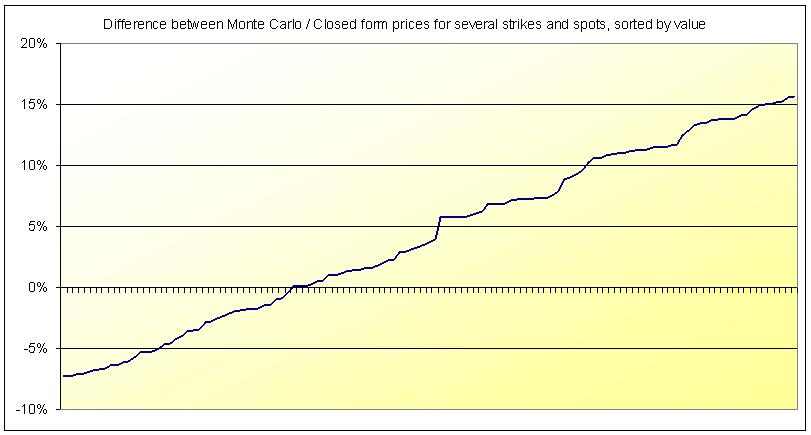
\includegraphics[width=14cm]{sobol.jpg}
        \caption{Prices differences using Sobol for best of's - Strikes and Spot moving between 50 and 150}
\end{center}
\end{figure}

This is of course unacceptable. We can refer to the article of Lee and Huang (Aletheia University) "Pricing Rainbow Options Using Monte Carlo Simulation - 2005" where they tested several random generators to price rainbows with Monte Carlo and showed that Sobol is not the best one to use, even in dimension 2 as it creates aggregates in some spaces of the unit cirle of $\mathbb{R}^2$.

We used VBA to price by Monte Carlo the rainbow and realized we had the correct prices with respect to the closed form. Moving to Mersenne Twister, we have (fig 8.2)

\begin{figure}
\begin{center}
        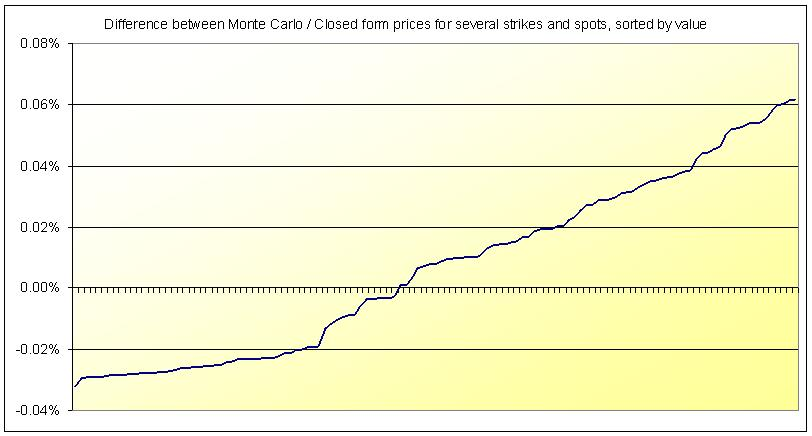
\includegraphics[width=14cm]{mersenne.jpg}
        \caption{Prices differences using Mersenne Twister for best of's - Strikes and Spot moving between 50 and 150}
\end{center}
\end{figure}

The differences do not exceed 8 basis points in relative absolute value, which is a very good thing.

We now had another issue. Indeed as we did not do the calculus for exact closed form value concerning the greeks, the method is finite difference. But Monte Carlo by itself converges to the prices but two different runs can lead to different prices. Hence assume the following: one it 2bps lower than the closed form and the other is 4 bps higher. Hence the greek calculation would be totally off. To calculate the greeks while bumping the reference parameter (spot, volatility, rate, etc) up and down, we have to make sure each set of paths faces the same states of the world, i.e. the same random samples, else it is completely off. We noted some deltas that should be 17 with closed form and that were swinging beween 5 and 500 depending on when we calculated them. We have to reset the seed of the random generator each time we use the engine, so as to make sure if we price exactly the same product with Monte Carlo, we get to exactly the same price. This has been done and here are the distribution of differences for the partial delta for the Best of, the Max Call and the Min Put (fig 8.3, 8.4 and 8.5).

\begin{figure}
\begin{center}
        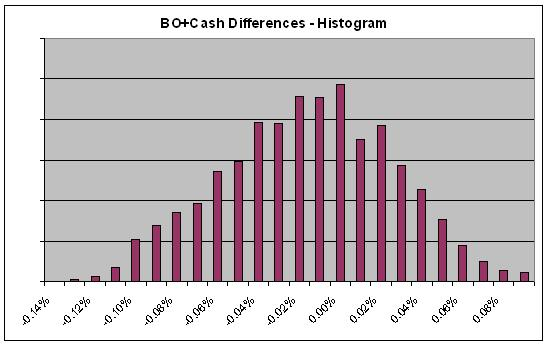
\includegraphics[width=14cm]{BOCPriceDiff.jpg}
        \caption{Distribution of delta differences Monte Carlo/Closed Form for the Best of, for different spots and strikes}
\end{center}
\end{figure} 

\begin{figure}
\begin{center}      
        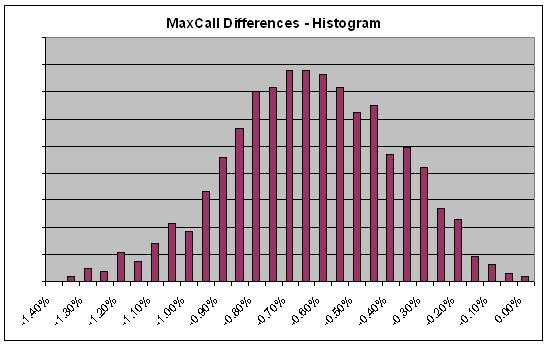
\includegraphics[width=14cm]{MaxCallPriceDiff.jpg}
        \caption{Distribution of delta differences Monte Carlo/Closed Form for the Max Call, for different spots and strikes}
\end{center}
\end{figure} 
  
\begin{figure}
\begin{center}    
        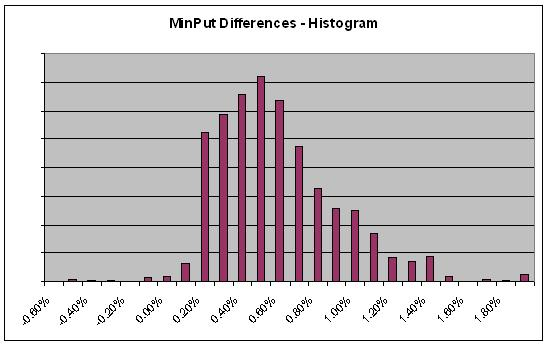
\includegraphics[width=14cm]{MinPutPriceDiff.jpg}
        \caption{Distribution of delta differences Monte Carlo/Closed Form for the Min Put, for different spots and strikes}
\end{center}
\end{figure}

At the end we have a very reliable object which the user can trust. As an example, here are a set of results we have for some products, and some prices as functions of the strike.

\begin{figure}
\begin{center}    
        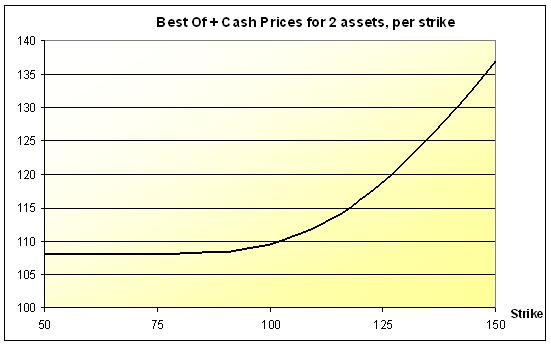
\includegraphics[width=14cm]{BOCPRice.jpg}
        \caption{Best of price as a function of the strike: $T=1$, $\s_1=\s_2=20\%$, $r=10\%$ and $S_1=S_2=100$}
\end{center}
\end{figure}

The very interesting noticeable fact is the importance of the rho as the strike gets higher. Indeed, in expectation, the stock prices in this case are $S_ie^{rT}\approx 110.5$, hence as we get tho higher strikes, the structure is likely to be close to a zero coupon bond, and be worth the discounted value of the strike. But then, the only risk we have on the product is a rate risk as we are virtually holding a ZCB. And holding a ZCB is being short the rates, meaning if rates move up, our structure is away from the fair value on the downside, and we are loosing money (fig 8.7).

\begin{figure}
\begin{center}    
        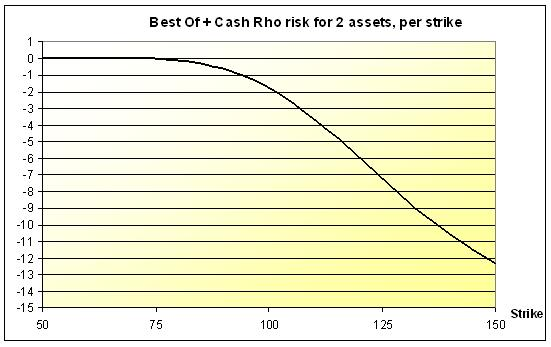
\includegraphics[width=14cm]{BOCRho.jpg}
        \caption{Best of rho as a function of the strike: $T=1$, $\s_1=\s_2=20\%$, $r=10\%$ and $S_1=S_2=100$}
\end{center}
\end{figure}

We also graphed the prices per strike in the same set of inputs for the 2 assets MAx/Min Call/Put's (fig 8.8)

\begin{figure}
\begin{center}    
        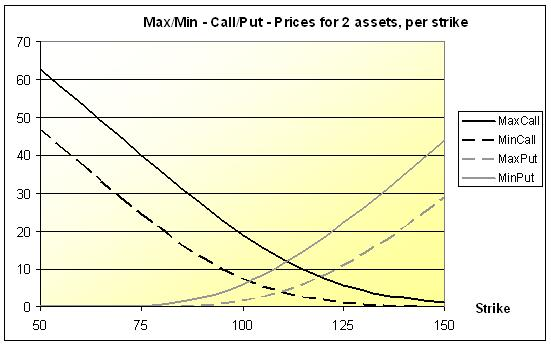
\includegraphics[width=14cm]{MAXMINCALLPUT2.jpg}
        \caption{Max/Min Call/Put's as functions of the strike: $T=1$, $\s_1=\s_2=20\%$, $r=10\%$ and $S_1=S_2=100$}
\end{center}
\end{figure}

As a set of results for the Best Of plus Cash, the MaxCall and the MinPut, we have run the Closed Form pricing range for the greeks, for a 2Y rainbow with $5\%$ interest rate. As both weights are identical, the partial with respect to both assets are equal. For the range of parameters, spots and strikes move in $[80,120]$, correlation in $[-1,1]$ and volatilities in $[10\%,30\%]$ The results are shown in table 8.9.

\begin{figure}
\begin{center}  
\begin{tabular}{|l|l|l|l|l|l|l|}
\cline{3-7}
\multicolumn{1}{l}{} &  & \multicolumn{1}{c|}{Partial Delta} & \multicolumn{1}{c|}{Partial Gamma} & \multicolumn{1}{c|}{Partial Vega} & \multicolumn{1}{c|}{Rho} & \multicolumn{1}{c|}{Correl} \\ 
\hline
Best Of & Min & \multicolumn{1}{r|}{0.32} & \multicolumn{1}{r|}{0.00} & \multicolumn{1}{r|}{0.01} & \multicolumn{1}{r|}{-42.39} & \multicolumn{1}{r|}{-16.40} \\ 
\cline{2-7}
 & Max & \multicolumn{1}{r|}{109.53} & \multicolumn{1}{r|}{520.09} & \multicolumn{1}{r|}{18.74} & \multicolumn{1}{r|}{0.00} & \multicolumn{1}{r|}{10.45} \\ 
\hline
MaxCall & Min & \multicolumn{1}{r|}{0.00} & \multicolumn{1}{r|}{0.00} & \multicolumn{1}{r|}{0.06} & \multicolumn{1}{r|}{8.84} & \multicolumn{1}{r|}{-15.59} \\ 
\cline{2-7}
 & Max & \multicolumn{1}{r|}{116.93} & \multicolumn{1}{r|}{519.42} & \multicolumn{1}{r|}{18.91} & \multicolumn{1}{r|}{28.28} & \multicolumn{1}{r|}{7.84} \\ 
\hline
MinPut & Min & \multicolumn{1}{r|}{-61.63} & \multicolumn{1}{r|}{0.10} & \multicolumn{1}{r|}{0.02} & \multicolumn{1}{r|}{-21.71} & \multicolumn{1}{r|}{-16.40} \\ 
\cline{2-7}
 & Max & \multicolumn{1}{r|}{0.00} & \multicolumn{1}{r|}{192.37} & \multicolumn{1}{r|}{4.33} & \multicolumn{1}{r|}{-2.29} & \multicolumn{1}{r|}{3.82} \\ 
\hline
\end{tabular}
	\caption{A few results on the greeks - Min and Max values noticed for reasonable parameters}
\end{center}
\end{figure}

It confirms the general intuition in which of course the Best of works as a call so it is long delta like the call, the put being short delta. All these are long gamma, as the single stock european versions, as well as long vega, which is understandable as when you own them, if the implied volatility goes up, their value appreciates. The rho is also logical: short for the best of + cash as explained, long for the call and short for the put, as for the european Black-Scholes options. And as for the correlation, depending on whether one spot is higher than the other, and whether their base correlation is positive or negative, the correlation risk can have a positive or a negative impact. Indeed, say we have a Max Call, if the base correlation is positive and high, the maximum is likely to be higher, so is the price: when the correlation decreases, it decreases the price.

Track of the results can be found in the data directory in rainbow2\_yann.xls, rainbow\_MC\_yann.xls and resRainbow\_yann.xls.

\section{Choices}
%<any important design choices you made, e.g. data structures, class hierarchy, algorithm, etc. and a justification for the decision>

We chose not to use dividends in the whole project (from Black-Scholes to the rainbows), but we could easily add them in our closed forms as shown earlier, and to Monte Carlo by adjusting the drift class and removing the dividend rate from the risk free growing rate. We had to amend the Drift/Gaussian/Random/MCEngine/Payoff classes in default constructors so as to avoid passing valarrays all the time and be more efficient: with non path dependant options, the only simulated point is the terminal one, so a one period model does not need to pass arrays of one parameter.

The choice was made to enable $n$ assets, so that adding a new type does not change the whole stucture of the class, and just needs adding the relevant pricing method to the class.




\section{Validation}


\subsection{Approach}

%<i.e. what alternate method was used to validate the results - if this required a lot of code then similar outline as above should apply>
To validate the results of this part even further, the only possibility was to recreate a monte carlo pricer with an easire structure, 
making it easier not to make bugs inside. For this we chose to dewvelop it in VBA. Since we also had closed formulas for some options 
we were quite confident with the results of our C++ pricer, but for some options, it was comfortable to get the same results with 
another pricer. This pricer can be found in the data part of our project under the name RainbowMCTests\_simon.xls. 
The user can input his own parameters in the spreadsheet, choose the number of simulations to run, a maximum acceptable error and 
can then run the simulation. One has to be careful since the program is much slower in VBA. After the calculation is finished 
there is a cell indicating TRUE on a yellow background if all tests passed or FALSE on a red background if some failed. We were happy 
to check that all results were really good and very close to our c++ results, even for a small number of generations.


%<i.e. what bugs were found>

\chapter{Part J: Convertible Bonds}
Developer: Aloke Mukherjee

\noindent Validator: Jospeh Perez


%DEVELOPER WRITES THIS PART --->

\section{Requirements}

%<description of the problem being solved, relevant equations, algorithms, etc>
A convertible bond behaves as a hybrid between a bond and a stock
because in addition to the principal guarantee and coupons it can
also be converted into a specified number of shares of stock at
given times.  As the chance of converting increases due to stock
price appreciation the price of convertible bonds will behave more
like the stock.  If the chance of converting is low then the
convertible's price will be more affected by interest rates and its
behaviour is more bond-like.

This "early-exercise" feature of convertible bonds makes it
difficult to model with Monte Carlo simulation.  Instead a binomial
tree is used to model the underlying stock price.  The convertible
bond is then evaluated at leaf nodes as the maximum of the par value
and the conversion value and these values are propagated back to the
tree's root.

An additional complication is the callability and putability
features of convertible bonds.  Callability allows the issuer to
call back the bond at a set price.  Putability conversely allows the
owner the put the bond back to the issuer at a set price.  This
optionality can also be modelled in the binomial tree by evaluating
at each step whether it is optimal for either party to exercise
their option.

\section{Design }

We constructed a binomial tree class which can store the
intermediate stock process and claim process values.  At
instantiation this class uses the yield curve and the stock's price
and volatility to calculate and cache the magnitude of each up and
down jump. The Cox-Ross-Rubinstein values are used - namely up moves
are $e^{\sigma\surd t}$ and down moves are the reciprocal of this.
The probability of an up move is the difference between the riskfree
value at the next node and the down value divided by the difference
between the up and down values.  The probability of a down move is
the complement.  We use the yield curve's ability to compute forward
discount factors to compute discount factors and probabilities for
each step of the tree.  If a flat yield curve is specified these
will all be the same but the design allows the use of a more
realistic yield curve.

Evaluation of the claim process is based on the same technique used
in the Monte Carlo simulation: different "Engine" methods are
defined in the binomial tree class which can be used to evaluate
different claim processes. The engine uses a standard PayOff object
used throughout the project to evaluate the claim at terminal nodes.
The engine applies risk-neutral probabilities to discount the payoff
as well as evaluating the different options at each node.  For
convertible bonds this decision can be expressed as 
$$max (Conversion\ value, min (Bond\ Value, Call\ Price), Put\ Price)$$

The convertible bond class' main task is to contain the various
attributes of the convertible such as conversion ratio, call price,
put price, the underlying asset and underlying risky bond.  Most
importantly it takes care of instantiating and invoking binomial
trees to calculate the price of the convertible as well as the
associated greeks.

\section{Choices}
%<any important design choices you made, e.g. data structures, class hierarchy, algorithm, etc. and a justification for the decision>

We made a few simplifying assumptions due to time constraints.  The
design is such that incorporating these factors in the future should
be straightforward.  As in other sections of the project we ignore
the effect of dividends.  The bond component of the convertible is
assumed to be a zero-coupon bond (e.g. no coupons). We assume that
callability and putability decisions are taken at each node in the
binomial tree.  Credit considerations are also neglected although
the convertible currently does take a credit curve in its
constructor.  This means that the "bond floor" will be slightly
higher than expected.

The convertible bond class inherits from the riskybond class.  This
makes sense intuitively because of its bond-like characteristics and
the fact that convertible's are issued by companies that have
default risk.  The binomial tree is implemented using arrays of
valarrays.  This simplifies instantiation and other operations
requiring access to the interior nodes.

The convertible bond greeks were calculated by comparing the given
convertible bond with a newly instantiated convertible bond with
appropriately shifted parameters.  The greeks calculated were:
\begin{itemize}
	\item $delta$ - change in convertible price corresponding to a change in
the price of the underlying asset.
	\item $gamma$ - change in delta corresponding to a change in the price of
the underlying asset.
	\item $rho$ - change in convertible price corresponding to a change in the
underlying interest rate. This was modelled by using the ability to
create a "shifted" risky bond with the yield curve shifted up by a
given number of points. Also referred to as interest rate delta.
\end{itemize}


Convertible greeks are often computed with respect to parity, the
product of conversion ratio and stock price.  Parity delta can be
computed by dividing delta by the adjusted conversion ratio and
parity gamma by dividing gamma by the square of the adjusted
conversion ratio.  The adjusted conversion ratio is simply the
conversion ratio scaled down by (face value / 100).  This allows the
parity greeks to be compared among bonds of differing face values.

Interestingly, convertibles have a few other greeks specific to
them.  One of these is omicron, the change in convertible price due
to a change in credit spreads.  Unfortunately, since we did not
model credit spreads in our pricing model we were not able to
compute this value.

\section{Unit tests}

%<short descriptions of each subtest>
The binomial tree class was verified by comparison with the Matlab
implemented binomial tree (discussed also in the Black-Scholes
section).  The Matlab code can be found in the data directory in the
file bintree.m.

In addition we verify in the C++ test that the most extreme leaf
nodes have the expected values given the specified volatility.
Finally we implemented an engine to evaluate a European claim.  This
value was compared to the results of the closed-form equations and
Monte Carlo simulation.  The binomial tree also has an output
operator which allows all the interior nodes of both the stock and
claim process to be displayed.  This was invaluable in verifying
correct operation.

The convertible bond was tested by trying out an example similar to
that outlined in Hull example 21.1 (6th edition).  This example has
similar assumptions to those outlined above except for the modeling
of default.  We find the price from our model is slightly higher
than that computed in Hull due to this simplification.  By
inspecting interior nodes we verified that the appropriate action
(e.g. call, put, conversion) predicted in Hull was chosen at each
interior node.  We also priced the Atmel convertible bond described
in the lecture notes.  Since we did not model all the parameters and
did not know the underlying yield curve the results did not match
exactly but they appeared to be in the ballpark.  The output of
these tests can be seen in the convertible test function accessible
from the test selection of the menu.

The convertible bond was also validated using Zhi Da's Convertible
Bond Calculator

(see http://www.kellogg.northwestern.edu/faculty/da)

which can be easily programmed to match the assumptions in our
model.  This is discussed further in the validation section but we
find the results to match well.  A copy of the calculator can be
found in the data directory as CBCalculator.xls.  It has been
slightly altered to not convert the specified rate into a continuous
rate.  It has also been loaded with the data used in the first
example in the convertible bond test.

\section{Performance}

%<how can the performance of this component be sped up by 100%?>
The binomial tree implementation can be optimized by a variety of
means.  Some of these are outlined in the paper "Nine Ways to
Implement the Binomial Method for Option Valuation in MATLAB"
(http://epubs.siam.org/sam-bin/getfile/SIREV/articles/39326.pdf).
The most important improvement suggested is using high-level
operations on arrays.  Matlab is specialized to deal with such
arrays however the same logic can be applied to C++ when using
valarrays since valarrays are optimized to handle batch operations
on all elements as in Matlab.  Space usage is also inefficient in
our implementation increasing with the square of the number of
steps.  The same calculations can be implemented using a single flat
array by replacing the elements as we work backwards through the
tree.

The convertible bond makes some use of caching.  It will cache the
price and greeks for the most recently requested date.  An
improvement here would be to implement some kind of hashmap allowing
these values to be cached for multiple dates.  Currently for example
if requests were made sequentially at different dates, the caching
functionality would not help.

%VALIDATOR WRITES THIS PART --->

\section{Validation}

\subsection{Approach}

To validate we run pricing of convertible bond with VBA. The excel
file is CBcalculator.xls (details above). The principle for pricing
is also to use a binomial tree. Giving the same parameters we got
the same results.

\begin{figure}
\begin{center}
        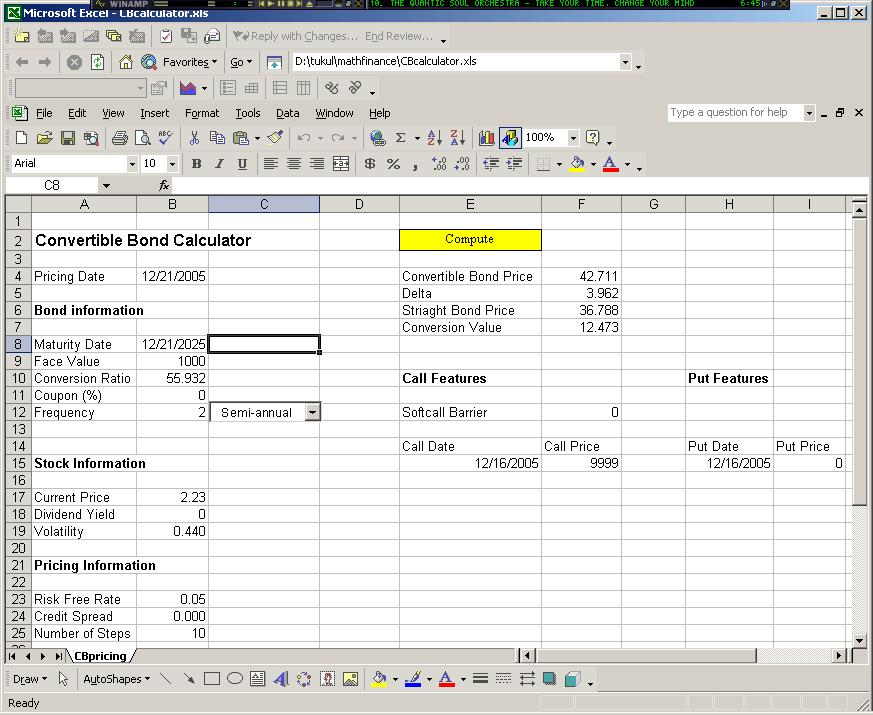
\includegraphics[width=12cm]{cbexample.jpg}
        \caption{Results of pricing of a convertible bond with VBA}
\end{center}
\end{figure}
\begin{figure}
\begin{center}
        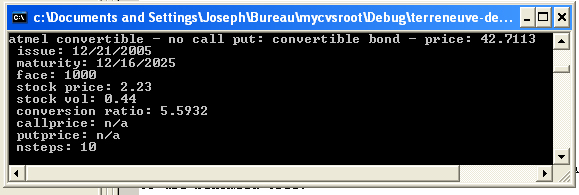
\includegraphics[width=12cm]{cbexample2.jpg}
        \caption{Results of pricing of a convertible bond with our project}
\end{center}
\end{figure}

%\subsection{Pitfalls}

%<i.e. what bugs were found>

\chapter{Part K: Variance Swaps}
Developer: Simon Leger

\noindent Validator: Aloke Mukherjee


%DEVELOPER WRITES THIS PART --->

\section{Requirements}

%<description of the problem being solved, relevant equations, algorithms, etc>
In this section, we use a portfolio of European options to compute
the value of a variance swap. We write methods to compute the value of such swaps.


\section{Design }

The value of a variance swap is computed according to the theoritical formula. 
There is in fact a formula to compute the value of a variance swap under 
no-arbitrage assumption which is not the case for volatility swaps for instance.

\section{Approach}
%<high-level description of the design>
To create a variance swap object, we use the OptionStrategy design
built in part A and we pass a pointer to such an object, with a
maturity and a forward price since it is all we need to compute
the value.


\section{Choices}
%<any important design choices you made, e.g. data structures, class hierarchy, algorithm, etc. and a justification for the decision>
We decided to create all information required in the constructor
of the object and store them like pointers so we have a function
getPrice() which calculates the price according to the values
stored and according to the following formula :

$$Price=\frac{2}{T}\left(\int_0^F\frac{1}{K^2}P(K)dK+\int_F^\infty \frac{1}{K^2}C(K)dK\right)$$

where $T$ is the maturity of the contract, $F$ is the forward price,
$P(K)$ is the price of the put and $C(K)$ the price of a call with
strikes $K$.


\section{Unit tests}

%<short descriptions of each subtest>
Test on the VIX index : To test the accuracy of the variance swap implementation 
we create a portfolio of puts and calls options, by using the OptionStrategy class. 
We take a minimum and a maximum strike and a step for this and we create a bench of options 
with these strikes, calls if the strike is higher than the forward value of S\&P and puts in the other case. 
With a minimum strike of 500, a maximum strike of 3500, a step of 10, we take a spot at 1200, the one month 
interest rate is around 4.3% and we assume a flat volatility of 33%, we get a price of 10.9, which is very close to 
the current value of the VIX index which is around 11.



%VALIDATOR WRITES THIS PART --->

\section{Validation}


\subsection{Approach}

%<i.e. what alternate method was used to validate the results - if this required a lot of code then similar outline as above should apply>
For this section's validation, the more efficient way to test the accuracy of the results provided bt 
the variance swaps part was to build the formula in an Excel spreadsheet built from prices of options, 
both calls and puts whose values have been calculated with the Black Scholes closed formula. We then compute 
the same price as in the example provided in the unit test part and we found the same result.
As well as for the VIX index, where we have very similar prices to exact value of the index found 
on the CBOE web site, such that we can consider that the results provided by this class are good.

\chapter{Part L: Exotic Products}
Developer: Simon Leger

\noindent Validator: Yann Renoux


%DEVELOPER WRITES THIS PART --->

\section{Requirements}

%<description of the problem being solved, relevant equations, algorithms, etc>
In this section, we design and write a monte carlo based framework that will allow us to price a variety of exotic products. Our framework has to be able to generate
simulateed paths for one asset, for every month for five years. Once we have these paths we apply a corresponding payoff formula on the set of paths to get a price for European style products with the following features :
\begin{itemize}
	\item Asian options
	\item Barrier options
	\item Look back options
	\item Cliquet
\end{itemize}


\section{Design }

To design this part, we chose to create just one class which is going to use the 
monte carlo based framework developed in part A. Then we add methods to get the price of the 
exotic according to a type associated with a given payoff and methods to get the greeks.

\section{Approach}
%<high-level description of the design>

The Monte-Carlo framework meets all requirements for this part. It is even more general
since we are able to generate as many intermediate points as we want for given dates.
As all these products have only one underlying, we are able to use the Sobol generator for them and we get better prices with it.

\section{Choices}
%<any important design choices you made, e.g. data structures, class hierarchy, algorithm, etc. and a justification for the decision>
This section is in the "Exotics" class. It takes in the constructor everything it requires to compute the price, they are stored as pointers also 
to make it faster and it also needs a type, which is the kind of products you need.
Here are all possibilities :

enum exoticsType {
\begin{itemize}
	\item AsianCall,
	\item AsianPut,
	\item RevLookbackCall,
	\item RevLookbackPut,
	\item FlooredCliquet,
	\item CappedCliquet,
	\item CollaredCliquet,
	\item BarrierCall,
	\item BarrierPut
\end{itemize}
};	

If one wants to add other products, this is very easy since he only needs to add a case in the getPrice() function and write a main montecarlo function for this and applying a new payoff.
We also provide the greeks by finite difference method. For this one needs to be careful 
since we have to apply the same random numbers to the paths to get correct greek values, other wise the 
Monte Carlo approximation error is greater than the difference given by the change on underlying, vol... depending on 
the greek value. For this we just reset the seed of the generator, which for Sobol is equivalent to recreate orginal 
vectors for it, which is done by creating a new instance of the generator. This is not a 
problem in terms of speed since we do not do any computation that is not required.


%VALIDATOR WRITES THIS PART --->

\section{Validation}


\subsection{Approach}

As these exotic derivatives do not have any closed form solution, our only alternate method to validate the prices is to use an independant Monte Carlo engine and recompute some prices for each option with different sets of parameters. As we had already designed a VBA based Monte Carlo tool, we re-used it to adapt it to the exotic payoffs, this time on a single asset but with path dependancy. Here then the simulated path should be a natural divider of the number of points needed in the payoff. Say for example that we consider a Reverse Look-Back of 2 years, with one added observation date after the first year, we need to simulate the path the end of year 1 AND the end of year 2 to be able to maximize the underlying price on these two dates. The rest follows usual pricing methodology, i.e. making sure we simulate the price with normal independant samples if we have several dates, and recombine the price with the correct drift and volatility for the brownian motion. In practise the drift would be $exp((r-\half\s^2)\frac{T}{nb\_Obs})$ and for the gaussian $exp(\s\sqrt{\frac{T}{nb\_Obs}})$ from one observation date to the other. For the following inputs:

\begin{center}
\begin{tabular}{|l|l|}
\hline
Spot & 100 \\ 
\hline
K & 100 \\ 
\hline
$\s$ & $20\%$ \\ 
\hline
r & $5\%$ \\ 
\hline
T & 1 \\ 
\hline
nPaths &  $100,000$  \\ 
\hline
\end{tabular}
\end{center}

We have checked the prices for some of the products -- Monte Carlo simulation in VBA is really slow, so we could not do a broad range as for the rainbows. All available exotics were done except the cliquets. We checked that for a single date, the Asians and Reverse Look Backs lead to the Black Scholes closed form solutions, which is the case. As we increase the number of dates, the maximum on the path should be higher, hence the ReverseLook Back Call should be more expensive with more dates while the put version should be less expensive. For the Asians, the averaging smoothes the extreme values hence for 2 dates and more, the price is lower than the associated Black Scholes European Call/Put. For the one-touch options, the more the dates, the more likely we are to touch the barrier, hence a higher price.

\begin{center}
\begin{tabular}{|l|l|l|l|l|}
\cline{2-5}
\multicolumn{1}{l|}{} & \multicolumn{2}{c|}{\textbf{Terreneuve}} & \multicolumn{2}{c|}{\textbf{Excel}} \\ 
\hline
nDates & \multicolumn{1}{c|}{1} & \multicolumn{1}{c|}{2} & \multicolumn{1}{c|}{1} & \multicolumn{1}{c|}{2} \\ 
\hline
RevLookBackCall & \multicolumn{1}{c|}{10.425} & \multicolumn{1}{c|}{12.169} & \multicolumn{1}{c|}{10.425} & \multicolumn{1}{c|}{12.208} \\ 
\hline
AsianCall & \multicolumn{1}{c|}{10.425} & \multicolumn{1}{c|}{8.108} & \multicolumn{1}{c|}{10.432} & \multicolumn{1}{c|}{8.115} \\ 
\hline
RevLookBackPut & \multicolumn{1}{c|}{5.578} & \multicolumn{1}{c|}{2.855} & \multicolumn{1}{c|}{5.596} & \multicolumn{1}{c|}{2.894} \\ 
\hline
AsianPut & \multicolumn{1}{c|}{5.578} & \multicolumn{1}{c|}{4.451} & \multicolumn{1}{c|}{5.544} & \multicolumn{1}{c|}{4.486} \\ 
\hline
One Touch Call & \multicolumn{1}{c|}{0.532} & \multicolumn{1}{c|}{0.641} & \multicolumn{1}{c|}{0.533} & \multicolumn{1}{c|}{0.640} \\ 
\hline
One Touch Put & \multicolumn{1}{c|}{0.419} & \multicolumn{1}{c|}{0.546} & \multicolumn{1}{c|}{0.418} & \multicolumn{1}{c|}{0.543} \\ 
\hline
\multicolumn{1}{l}{} & \multicolumn{1}{c}{} & \multicolumn{1}{c}{} & \multicolumn{1}{c}{} & \multicolumn{1}{c}{} \\ 
\cline{1-2}
Black Scholes Call & \multicolumn{1}{c|}{10.451} & \multicolumn{1}{c}{} & \multicolumn{1}{c}{} & \multicolumn{1}{c}{} \\ 
\cline{1-2}
Black Scholes Put & \multicolumn{1}{c|}{5.574} & \multicolumn{1}{c}{} & \multicolumn{1}{c}{} & \multicolumn{1}{c}{} \\ 
\cline{1-2}
\end{tabular}\end{center}

The remarks on the moves of prices with the number of dates are met, as well as Black-Scholes comparison. The prices for only $100,000$ simulations are in line within $1.4\%$ (for the reverse look back put on 2 dates), so we can consider that this object passes the validation test. Result file in data/exotics\_yann.xls


\subsection{Pitfalls}

No major pitfall was found. As for the other classes, the on-going validation process enabled to discover some bugs that were fixed, and also for more than one date, do not use Sobol in one dimension.

\chapter{Part M: Portfolio}
Developer: All

\noindent Validator: All


%DEVELOPER WRITES THIS PART --->

\section{Requirements}

%<description of the problem being solved, relevant equations, algorithms, etc>
In this section we design and write a framework that represents the characteristics and behavior
 of portfolios and their values and risk under different types of market scenarios. Each portfolio 
has a name and a currency. All relevant financial information about the portfolio such as its value, 
profit/loss, and risk is expressed in the portfolio currency. The portfolio will contain a number of securities 
whose positions, profit loss and risk the objects will manage. For each security in the portfolio our framework will 
provide the security name, cost basis, current price, price currency amount, current value, profit loss.
Each security will have a risk profile called its risk map. The risk map describes the variation in the value of the 
security for changes/shifts in risk factors. The framework will allow scenario analysis for the portfolio. We should implement methods for the following :
\begin{itemize}
	\item Current value of the security
	\item Profit loss for the security
	\item Profit loss for the portfolio
	\item Current value of the portfolio
	\item Import portfolio information from a file
	\item Import list of securities from a file
	\item Import risk map of a security from a file
	\item Import scenario list from a file
	\item Value of the portfolio for a single risk factor risk scenario
	\item Profit/Loss report
	\item Portfolio analysis report
	\item Value at risk for the portfolio
\end{itemize}

\section{Choices }

As mentionned by Pr Laud in the last week, we did not try to do the VaR. Though the framework of the project would have easily permitted it, we have chosen to focus on validating correctly all the delivered structures rather than delivering more but not being sure of the reliability of the products.

The design enables the structure to be able to handle the requirements as if bears all the information on all the products we developped in this project.

\section{Approach}
%<high-level description of the design>
The portoflio class in the C++ project just takes a name and a currency and provides the user of the program with methods to add 
each type of security we have, namely :
\begin{itemize}
	\item OptionStrategy, which is already a portfolio of BlackScholes object
	\item Rainbow options
	\item Exotic options
	\item Vanilla swap
	\item Variance swap
	\item Bond
	\item Asset
\end{itemize}

There is also a method to compute the value of the portfolio and to get the absolute risk for different sorts of scenarios, similar to the greeks for the options.

\section{Choices}
%<any important design choices you made, e.g. data structures, class hierarchy, algorithm, etc. and a justification for the decision>
Each security is stored in the portfolio in valarrays of pointers to these objects, since we dont want to make a copy of already existing objects. For each security we also have a quantity, in order to avoid to copy them many times in the portfolio.
\par We also provide similar methods to greek values for the portfolio, giving a risk value for different kinds 
of risks, which are calculated by calling these methods from the security class, if this one exists. For example there is no sensibility 
to volatility for a bond or a vanilla IR swap, but each security has a sensibility to the interest rate or to time.



%VALIDATOR WRITES THIS PART --->

\section{Validation}

All structures were validated in the other sections, and tested. This one just goes through all the valarrays of the products to add them (deleting is adding the opposite quantity) and return the value of the portfolio, and its greeks with which we could output the stress loss or PnL report based on the moves of any market parameter.
\chapter{Conclusion}

\par This report is quite long, so we will not spread pages as a conclusion.

We obviously learnt a lot with this project, as we have tried to share a lot on the issues we were facing on a daily basis. The number of emails of the list that were sent per day is amazingly huge. 

It leads us to the fact that the team work was excellent on this project, and the use of CVS and Skype for conference calls -- we said we thanked the nerds that invented the internet ! -- made sure that from the beginning the objects were plugging together exactly. We avoided much of the last minute pain in doing that.

We hope the project is in the most deliverable state as possible, even if the user cannot "consolely" play with all the products, the code is there anyways.

\bigskip

\textbf{Future Work}

This project clearly illustrates the complexity of the universe of financial products.  Additionally, there can be many approaches to modelling each product. In this project we have implemented some of the most popular modeling techniques including closed-forms, Monte Carlo simulation and binomial trees, and not just in C++ but also in Excel and Matlab! As developers attempting to work with this variety, the first and foremost imperative is "get it working". 
We've learned that this is not a simple task: to begin with how will you even know it is working? But once you've conquered that peak, the sky is the limit: approaches can be changed, parameters altered, models made more precise, computations made more efficient. This project has been a great experience because it has exposed us to a wide variety of approaches and techniques. And having not died from exposure, we can see from these heights how much exciting work there is left to do!

\bigskip

\bigskip

-- The Terreneuve Team that will now celebrate as a team the end of the semester.


%call each file PartX.tex and then add here \input{PartX.tex}


\end{document}
